%
%%%%%%%%%%%%%%%%%%%%%%%%%%%%%%%%%%%%%%%%%%%%%%%%%%%%%%%%%%%%%%%%%%%%%%
%%%%%%%%%%%%%%%%%%%%%%%%%%%%%%%%%%%%%%%%%%%%%%%%%%%%%%%%%%%%%%%%%%%%%%%
%%%%%%%%%%%%%%%%%%%%%%%%%%%%%%%%%%%%%%%%%%%%%%%%%%%%%%%%%%%%%%%%%%%%%%%
%%%%%%%%%%%%%%%%%%%%%%%%%%%%%%%%%%%%%%%%%%%%%%%%%%%%%%%%%%%%%%%%%%%%%%%
\chapter{Parameter, Covariate and Observation Models}
\label{ch:Models}


%%%%%%%%%%%%%%%%%%%%%%%%%%%%%%%%%%%%%%%%%%%%%%%%%%%%%%%%%%%%%%%%%%%%%%
\section{Distribution type -- new model type}
\label{sec:newModelType}
The new model type follows the textbook notation for definition of the distribution 
of a random variable and can be applied for covariates, parameters, observations etc.
It is required when defining e.g. a parameter model without the detour
of using a random effect (sometimes called the \emph{eta-free} notation). 
\begin{itemize}
\item
Distribution type
\begin{align*}
	h(X) & \sim DistributionName(parameter1, parameter2, \dots) 
\end{align*}
e.g. 
\begin{align*}
\log(X) & \sim \mathcal N\big(\log(X_{typical}), \omega_X\big)
\end{align*}
with X standing for a covariate, parameter, observation etc. Examples 
will be given below.
\end{itemize}
This type can be encoded using both ProbOnto or 
UncertML although the latter option has limitations compared to ProbOnto, 
described in detail in section \ref{sec:uncertmlLimits}, in that it doesn't allow 
to encode arbitrary expressions as parameters, as required in the above example.

%%%%%%%%%%%%%%%%%%%%%%%%%%%%%%%%%%%%%%%%%%%%%%%%%%%%%%%%%%%%%%%%%%%%%%
\section{Individual parameter representations -- extended}
\label{sec:individualParameter}

Following changes have been introduced to cover a broader class of parameter models
\begin{itemize}
\item
\xelem{GaussianModel} element has been renamed to \xelem{StructuredModel} to account
for its general purpose, beyond the normal distribution, an example follows below. 
\item
\xelem{PopulationParameter} element has been renamed to \xelem{PopulationValue} 
for consistency with its meaning and use.
\item
\xelem{Transformation} element has been redesigned in order to account for
Box-Cox transformation (see Section \ref{sec:BoxCoxTrafo} for a description).
Instead of 
\lstset{language=XML}
\begin{lstlisting}
                <StructuredModel>
                    <Transformation>log</Transformation>
\end{lstlisting}
now it reads
\lstset{language=XML}
\begin{lstlisting}
                <StructuredModel>
                    <Transformation type="log"/>
                    ...
\end{lstlisting}
with \xatt{type} to be assigned one of the values: \{idenitity, log, logit, probit, BoxCox\footnote{introduced in Section \ref{sec:BoxCoxTrafo}}\}
\item
\xelem{PopulationValue} can be used without the parent element 
\xelem{LinearCovariate} if no covariate is taken into account.
E.g. for the simplest case of a log-normally distributed parameter $\log(V) = \log(V_{pop}) + \eta_V$
the following completely describes the model and is shown in two equivalent versions,
table \ref{tab:missingCovariateModel}.
\begin{table}[ht!]
\setlength{\tabcolsep}{5pt}
\begin{center}
\begin{tabular}{cc}
  \hline
  \hline
{\color{red} \scshape{NEW}} without \xelem{LinearCovariate} element  & with \xelem{LinearCovariate} element \\
  \hline
\lstset{language=XML}
\begin{lstlisting}
<IndividualParameter symbId="V">
   <StructuredModel>
       <Transformation type="log"/>
       <PopulationValue>
          <ct:Assign>
             <ct:SymbRef symbIdRef="Vpop"/>
          </ct:Assign>
       </PopulationValue>
       <RandomEffects>
          <ct:SymbRef symbIdRef="eta_V"/>
       </RandomEffects>
   </StructuredModel>
</IndividualParameter>
 \end{lstlisting}
&
\lstset{language=XML}
\begin{lstlisting}
<IndividualParameter symbId="V">
  <StructuredModel>
      <Transformation type="log"/>
      <LinearCovariate>
         <PopulationValue>
             <ct:Assign>
                 <ct:SymbRef symbIdRef="Vpop"/>
             </ct:Assign>
         </PopulationValue>
      </LinearCovariate>
      <RandomEffects>
         <ct:SymbRef symbIdRef="eta_V"/>
      </RandomEffects>
  </StructuredModel>
</IndividualParameter>
\end{lstlisting}  \\
  \hline
  \end{tabular}
\vspace{-1.5em}
\caption{Comparison of equivalent implementation of the basic parameter model,
$\log(V) = \log(V_{pop}) + \eta_V$, without a covariate. The element \xelem{PopulationValue}
doesn't have to be nested within \xelem{LinearCovariate} as was the case in $\leq$ 0.6.}
\label{tab:missingCovariateModel}
\end{center}
\end{table}

%\lstset{language=XML}
%\begin{lstlisting}
%            <IndividualParameter symbId="V">
%                <StructuredModel>
%                    <Transformation type="BoxCox">
%                        <Lambda>
%                            <ct:Assign>
%                                <ct:SymbRef symbIdRef="lambda"/>
%                            </ct:Assign>
%                        </Lambda>
%                    </Transformation>
%\end{lstlisting}
\end{itemize}
The following representations types are available 
\begin{description} 
\item[Type I1]  Structured (e.g. Gaussian) model 
\begin{itemize}
\item
	A.  Linear covariate model
\begin{align*}
         	h(\psi_i) = h(\psi_{pop}) + \beta c_i + \eta_i \quad [\text{Gaussian if } \eta_i \sim N(.,.)]
 \end{align*}
               
\item
	B. General covariate model
\begin{align*}
        	h(\psi_i) = H(\beta, c_i) + \eta_i  \quad [\text{Gaussian if } \eta_i \sim N(.,.)]
\end{align*}
\end{itemize}
\item[Type I2] Equation type
\begin{align*}
       		\psi_i = H(\beta, c_i, \eta_i)
\end{align*}    
\item[Type I3] ({\color{red} \scshape{NEW}}) Distribution type (i.e. eta-free notation)
\begin{align*}
		& h(\psi_i) \sim DistributionName(parameter1, parameter2, \dots)
\end{align*}
\end{description}

\begin{example}
Individual model as used in the formulation of a hierarchical model example
proposed in \cite{LavielleFourModels:2014}
\begin{align*}
		&\log(\psi_i) \sim \mathcal {LN}\big(V_{pred}, \omega_V\big) 
\end{align*}

\lstset{language=XML}
\begin{lstlisting}
            <IndividualParameter symbId="V">
                <LHSTransformation type="log"/>
                <ct:VariabilityReference>
                    <ct:SymbRef blkIdRef="vm1" symbIdRef="indiv"/>
                </ct:VariabilityReference>
                <Distribution>
                    <ProbOnto name="LogNormal1">
                        <Parameter name="meanLog">
                            <ct:Assign>
                                <ct:SymbRef symbIdRef="V_pred"/>
                            </ct:Assign>
                        </Parameter>
                        <Parameter name="stdevLog">
                            <ct:Assign>
                                <ct:SymbRef symbIdRef="omega_V"/>
                            </ct:Assign>
                        </Parameter>
                    </ProbOnto>
                </Distribution>
            </IndividualParameter>
\end{lstlisting}
\end{example}

\begin{note} \xelem{StructuredModel} extends \xelem{GaussianModel} to be more general
without loosing the ability to express the later -- this updated element allows e.g. Student-T 
distributed parameters to be formulated in the additive form
\begin{align*}
                \log(V_i) = \log(V_{pop}) + \beta c_i + \eta_i, \quad \text{with} \quad \eta_i \sim StudentT(0,\omega_V)
\end{align*}
\end{note}

\begin{note}  New Distribution-type (Type 2B) allows using UncertML/ProbOnto 
to define a model without the random effect detour, e.g.
\begin{align*}
		\log(V_i) \sim \mathcal N\big(\log(V_{pop}), \omega_V\big) 		
\end{align*}
which is equivalent to 
\begin{align*}
                \log(V_i) = \log(V_{pop}) + \eta_i \quad \text{with} \quad \eta_i \sim \mathcal N(0,\omega_V)
\end{align*}
\end{note}

\begin{note}   ProbOnto, compared to UncertML, provides additional support for 
expressions in parameters, e.g. $mean = \log(V_{pop})$ in the above equation.
\end{note}

\begin{note} Type 2B comes with support for multiple levels of variability, Figure \ref{fig:IOVtree},
\begin{align*}
\log(V_{ik}) \sim \mathcal N\big(\log(V_{pop}), \underbrace{\omega_V}_{\text{\parbox{.8cm}{\centering IIV\\[-4pt] level 0}}} +  \underbrace{\kappa_V}_{\text{\parbox{.8cm}{\centering IOV\\[-4pt] level 1}}}\big)
\end{align*}
\end{note}


\begin{figure}[htb!]
\centering
 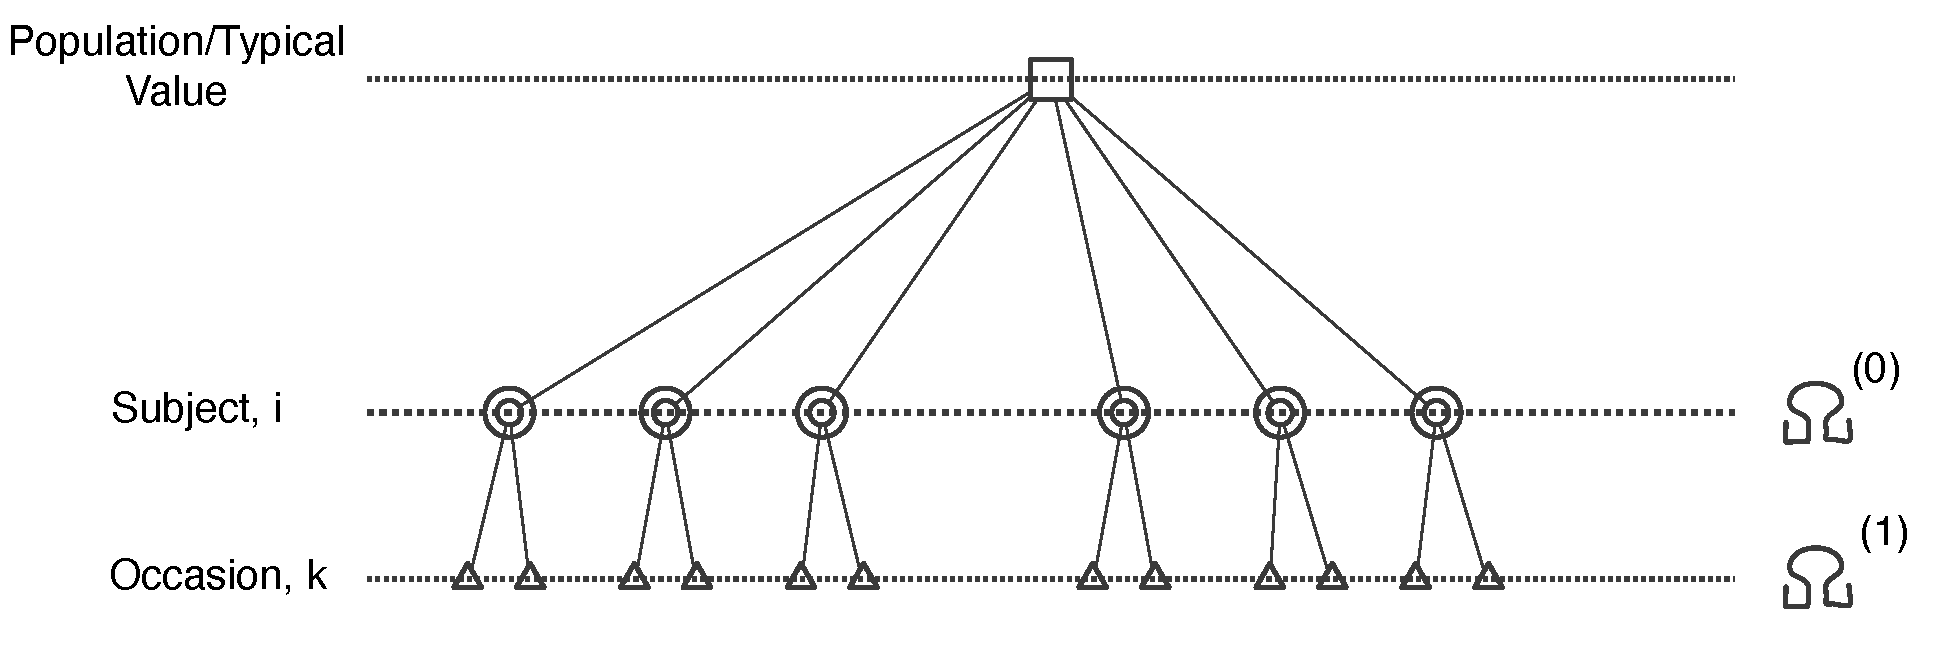
\includegraphics[width=120mm]{pics/IOV_2levels}
\caption{Model with IOV variability level.}
\vspace{-1em}
\label{fig:IOVtree}
\end{figure}


as the following PharmML snippet shows
\lstset{language=XML}
\begin{lstlisting}
            <IndividualParameter symbId="V">
                <ct:VariabilityReference>
                    <ct:SymbRef symbIdRef="iov"/>
                    <ct:RandomEffectMapping>
                        <ct:SymbRef symbIdRef="kappa_V"/>
                    </ct:RandomEffectMapping>
                </ct:VariabilityReference>
                <ct:VariabilityReference>
                    <ct:SymbRef symbIdRef="subject"/>
                    <ct:RandomEffectMapping>
                        <ct:SymbRef symbIdRef="omega_V"/>
                    </ct:RandomEffectMapping>
                </ct:VariabilityReference>
                <Distribution>
                    <ProbOnto name="Normal1">
                        <Parameter name="mean">
                            <ct:Assign>
                                <math:Equation>
                                    <math:Uniop op="log">
                                        <ct:SymbRef symbIdRef="Vpop"/>
                                    </math:Uniop>
                                </math:Equation>
                            </ct:Assign>
                        </Parameter>
                        <Parameter name="stdev">
                            <ct:Assign>
                                <math:Equation>
                                    <math:Binop op="plus">
                                        <ct:SymbRef symbIdRef="omega_V"/>
                                        <ct:SymbRef symbIdRef="kappa_V"/>
                                    </math:Binop>
                                </math:Equation>
                            </ct:Assign>
                        </Parameter>
                    </ProbOnto>
                </Distribution>
            </IndividualParameter>
\end{lstlisting}
The code above illustrates how 
\begin{itemize}
\item 
expressions can be encoded using ProbOnto,
here the $\log(Vpop)$ as the \emph{mean} parameter of the normal distribution.
\item
higher variability levels -- here the IOV -- by mapping of the according variances
to a particular level using the new \xelem{RandomEffectMapping} element. $\omega_V$
is mapped to IIV, $\kappa_V$ is mapped to IOV. Note, that the same information could 
have been implemented using the \xelem{StructuredModel}, but additionally two random 
effects would have to be declared.
\end{itemize}

%%%%%%%%%%%%%%%%%%%%%%%%%%%%%%%%%%%%%%%%%%%%%%%%%%%%%%%%%%%%%%%%%%%%%%
\section{Population parameter -- new}
\label{sec:populationParameter}
Population parameter comes with a flexible structure and can have an 
associated distribution, see Chapter \ref{ch:Bayesian} on Bayesian inference 
and hierarchical models.Two representations are available 
\begin{description} 
\item[Type P1] Equation type
\begin{align*}
\psi_{pop} = H(\beta_i, \eta_i, ...)
\end{align*}
\item[Type P2] Distribution type, i.e. eta-free notation 
\begin{align*}
	& h(\psi_{pop}) \sim Distribution(parameter1, parameter2, ...)
\end{align*}
%	 e.g.
%\begin{align*}
%	& \log(V_{pop}) \sim \mathcal N(\mu_{V_{pop}}, var_{V_{pop}})
%\end{align*}
\end{description}

\begin{note} 
\xelem{PopulationParameter} replaces the \xelem{SimpleParameter} which 
became redundant as the \marginpar{\HandCuffLeft} latter was used so far 
as a population parameter.
\end{note} 

\begin{example}
Using UncertML - from \emph{example3311.xml} model:
\begin{align*}
	lPOP_K \sim \mathcal N\big(lMU_{POP_K}, VAR_{POP_K}\big)
\end{align*}
is encoded in PharmML as
\lstset{language=XML}
\begin{lstlisting}
    <PopulationParameter symbId="lPOP_K">
        <ct:VariabilityReference>
            <ct:SymbRef symbIdRef="pop" blkIdRef="model"/>
        </ct:VariabilityReference>
        <Distribution>
            <UncertML>
                <NormalDistribution xmlns="http://www.uncertml.org/3.0" definition="">
                    <mean>
                        <var varId="lMU_POP_K"/>
                    </mean>
                    <variance>
                        <var varId="VAR_POP_K"/>
                    </variance>
                </NormalDistribution>
            </UncertML>
        </Distribution>
    </PopulationParameter>
\end{lstlisting}
\end{example}

\begin{example}
Using ProbOnto and Type P2 - from fourModels\_hierarchical.xml, \cite{LavielleFourModels:2014},
\begin{align*}
	V_{pop} \sim \mathcal {LN}\big(log(V\!s), gV\big)
\end{align*}
is encoded in PharmML as
\lstset{language=XML}
\begin{lstlisting}
            <PopulationParameter symbId="V_pop">
                <ct:VariabilityReference>
                    <ct:SymbRef blkIdRef="vm1" symbIdRef="pop"/>
                </ct:VariabilityReference>
                <Distribution>
                    <ProbOnto name="LogNormal1">
                        <Parameter name="meanLog">
                            <ct:Assign>
                                <math:Equation>
                                    <math:Uniop op="log">
                                        <ct:SymbRef symbIdRef="Vs"/>
                                    </math:Uniop>
                                </math:Equation>
                            </ct:Assign>
                        </Parameter>
                        <Parameter name="stdevLog">
                            <ct:Assign>
                                <ct:SymbRef symbIdRef="gV"/>
                            </ct:Assign>
                        </Parameter>
                    </ProbOnto>
                </Distribution>
            </PopulationParameter>
\end{lstlisting}
\end{example}

%%%%%%%%%%%%%%%%%%%%%%%%%%%%%%%%%%%%%%%%%%%%%%%%%%%%%%%%%%%%%%%%%%%%%%
\section{Observation model -- {\color{black} \scshape{extended}}}
\label{sec:observationModel}


\subsection{Discrete data models}
The new features are 
\begin{itemize}
\item
Seriously simplified encoding of discrete data models. In \pml versions $\leq$ 0.6 
the implementation of explicit PMF was required for many models due to the lack of 
their coverage in UncertML
\item
All common/relevant parametric distributions and/or their alternative parameterisations 
are supported by ProbOnto, as described in Chapter \ref{ch:ProbOnto}.
\item
Addition of new distributions is straightforward and will be done upon request
\item
As an example of ProbOnto use, we discuss here a complete observation model for count data
\begin{itemize}
\item
Type of observed variable -- discrete/count
\item
Model name: NegativeBinomial2
\item
Count variable: $y$
\item
Number of counts: $k$
\item
Probability mass function
\begin{eqnarray}
P(y_{ij} = k; \lambda, \tau) &=& \Bigg[ \frac{\Gamma \big( k + \frac{1}{\tau} \big)}{k! \times \Gamma \big(\frac{1}{\tau} \big)} \Bigg] \times \Bigg( \frac{1}{1 + \tau \times \lambda} \Bigg)^{\frac{1}{\tau}} \times \Bigg(\frac{\lambda}{\frac{1}{\tau} + \lambda} \Bigg)^k \nonumber
\end{eqnarray}
\item
Link function: $\log$
\item
Dispersion parameter, $\tau$
\item
Constant rate parameter $\lambda$, the Poisson 'intensity': $\lambda(t_{ij}, \psi_{ij}) = \lambda_{i}$
\end{itemize}
and reads in PharmML as
\lstset{language=XML}
\begin{lstlisting}
        <ObservationModel blkId="om2">
            <Discrete>
                <CountData>
                    <CountVariable symbId="y"/>
                    <NumberCounts symbId="k"/>
                    
                    <PMF linkFunction="log">
                        <math:LogicBinop op="eq">
                            <ct:SymbRef symbIdRef="y"/>
                            <ct:SymbRef symbIdRef="k"/>
                        </math:LogicBinop>
                        <ProbOnto name="NegativeBinomial2">
                            <Parameter name="rate">
                                <ct:Assign>
                                    <ct:SymbRef blkIdRef="pm1" symbIdRef="lambda"/>
                                </ct:Assign>
                            </Parameter>
                            <Parameter name="overdispersion">
                                <ct:Assign>
                                    <ct:SymbRef blkIdRef="pm1" symbIdRef="tau"/>
                                </ct:Assign>
                            </Parameter>
                        </ProbOnto>
                    </PMF>
                </CountData>
            </Discrete>
        </ObservationModel>
\end{lstlisting}
with \emph{lambda} and \emph{tau} defined in the parameter model, \xatt{pm1}
\end{itemize}


\subsection{Continuous data models}
\label{subsec:contModels}
Available observation model representation has been extended and the available types are
\begin{description} 
\item[Type O1] Structured model 
%(VariabilityReference not mandatory , RLHS required)
\begin{align*}
	u(y) = u(f) + g \times \epsilon \quad [\text{Gaussian if } \epsilon \sim \mathcal N(.,.)]
\end{align*}
is still used with the \xelem{Standard} tag (but comes with extended interpretation 
and allows non-Gaussian residual errors (see the related discussion in section 
\ref{sec:individualParameter}). Also the Box-Cox transformation can be applied 
in this case, see discussion in section \ref{sec:BoxCoxTrafo}.
\item[Type O2] General model (equation type), unchanged compared to 0.6
%(VariabilityReference not required, LHS transformation optional)
\begin{align*}
	h(y) = H(f, \xi, \epsilon)
\end{align*}

\item[Type O3] ({\color{red} \scshape{NEW}}) Distribution type ($\epsilon$-free notation) 
%(VariabilityReference required, LHS transformation optional)
\begin{align*}
	& u(y)  \sim DistributionName(parameter1, parameter2, ...)
\end{align*}

\end{description}

\begin{table}[ht!]
\setlength{\tabcolsep}{1pt}
\begin{center}
\begin{tabular}{cc}
  \hline
  \hline
\textbf{Type O1} representation  &  \textbf{Type O3} representation \\
  \hline
$Y = C + SD\_ADD \times \epsilon \quad \text{with} \quad \epsilon \sim \mathcal N(0,1)$ \Gape[.4cm][.2cm]{} 
& 
$Y  \sim \mathcal N(C,SD\_ADD)$
\\
  \hline
% \multicolumn{2}{c}{encoding [0,2,0,0,5,0,0,0,0,0]}  \\
%  \hline
  \lstset{language=XML}
\begin{lstlisting}
<Standard symbId="Y">
   <Output>
     <!-- blkIdRef="sm1" -->
     <ct:SymbRef symbIdRef="C"/>
   </Output>
   <ErrorModel>
     <!-- blkIdRef="pm1" -->
     <ct:Assign>
        <ct:SymbRef symbIdRef="SD_ADD"/>
     </ct:Assign>
   </ErrorModel>
   <ResidualError>
      <ct:SymbRef symbIdRef="eps"/>
   </ResidualError>
</Standard>
<!-- declaration of 'eps' omitted -->
\end{lstlisting}
&
\lstset{language=XML}
\begin{lstlisting}
<General symbId="Y">
   <ct:VariabilityReference>
      <ct:SymbRef symbIdRef="residual"/>
   </ct:VariabilityReference>
   <Distribution>
      <ProbOnto name="Normal1">
         <Parameter name="mean">
            <ct:Assign>
               <ct:SymbRef symbIdRef="C"/>
            </ct:Assign>
         </Parameter>
        <Parameter name="stdev">
            <ct:Assign>
               <ct:SymbRef symbIdRef="SD_ADD"/>
            </ct:Assign>
         </Parameter>
      </ProbOnto>
   </Distribution>
</General>
\end{lstlisting}  \\
  \hline
  \end{tabular}
\vspace{-1.5em}
\caption{Comparison of \textit{Type O1} and \textit{Type O3} ($\epsilon$-free) 
representations. For better code readability the \xatt{blkIdRef} attributes have 
been removed.}
\label{tab:typeComparison}
\end{center}
\end{table}


%\subsection{Model overview}
%
%\begin{table}[ht!]
%\setlength{\tabcolsep}{1pt}
%\begin{center}
%\begin{tabular}{cc}
%  \hline
%  \hline
%Individual parameter  & Population parameter \\
%  \hline
%\\
%  \hline
%  \lstset{language=XML}
%\begin{lstlisting}
%
%\end{lstlisting}
%&
%\lstset{language=XML}
%\begin{lstlisting}
%
%\end{lstlisting}  \\
%  \hline
%  \end{tabular}
%\vspace{-1.5em}
%\caption{Compilation of parameter models ...}
%\label{tab:modelCompilation}
%\end{center}
%\end{table}

%%%%%%%%%%%%%%%%%%%%%%%%%%%%%%%%%%%%%%%%%%%%%%%%%%%%%%%%%%%%%%%%%%%%%%
%%%%%%%%%%%%%%%%%%%%%%%%%%%%%%%%%%%%%%%%%%%%%%%%%%%%%%%%%%%%%%%%%%%%%%%
%%%%%%%%%%%%%%%%%%%%%%%%%%%%%%%%%%%%%%%%%%%%%%%%%%%%%%%%%%%%%%%%%%%%%%%
%%%%%%%%%%%%%%%%%%%%%%%%%%%%%%%%%%%%%%%%%%%%%%%%%%%%%%%%%%%%%%%%%%%%%%%
\chapter{Hierarchical models and Bayesian Inference}
\label{ch:Bayesian}

While the detailed Bayesian support is described in the according MDL 
specification proposal, \cite{Chiudinelli2015}, we describe here a few PharmML 
elements, either entirely new, redefined or as used in the context of 
hierarchical models and Bayesian inference.

\begin{itemize}
\item 
The \xelem{PopulationParameter} element provides, as indicated in section 
\ref{sec:populationParameter}, the support required for such models, i.e.
distribution notation.
\item 
ProbOnto provides missing distributions, such as \emph{Inverse-Wishart} 
and other features required. 
\item 
Prior related variability level of any parameter extends its variability 
structure used so far, see Figure \ref{fig:priorVM1}, and 
consequently the extended parameter related variability model for this 
case reads
\lstset{language=XML}
\begin{lstlisting}
        <VariabilityModel blkId="model" type="parameterVariability">
            <Level symbId="pop"/>
            <Level symbId="indiv">
                <ParentLevel>
                    <ct:SymbRef symbIdRef="pop"/>
                </ParentLevel>
            </Level>
        </VariabilityModel>
\end{lstlisting}
\item 
Few basic matrix operators, available as attributes of the new \xelem{MatrixUniOp} element 
-- such as \emph{inverse},  \emph{transpose}, \emph{trace} has been introduced to 
allow for encoding of related model features, see examples in the next section.
\end{itemize}


\begin{figure}[htb!]
\centering
\begin{tabular}{cc}
 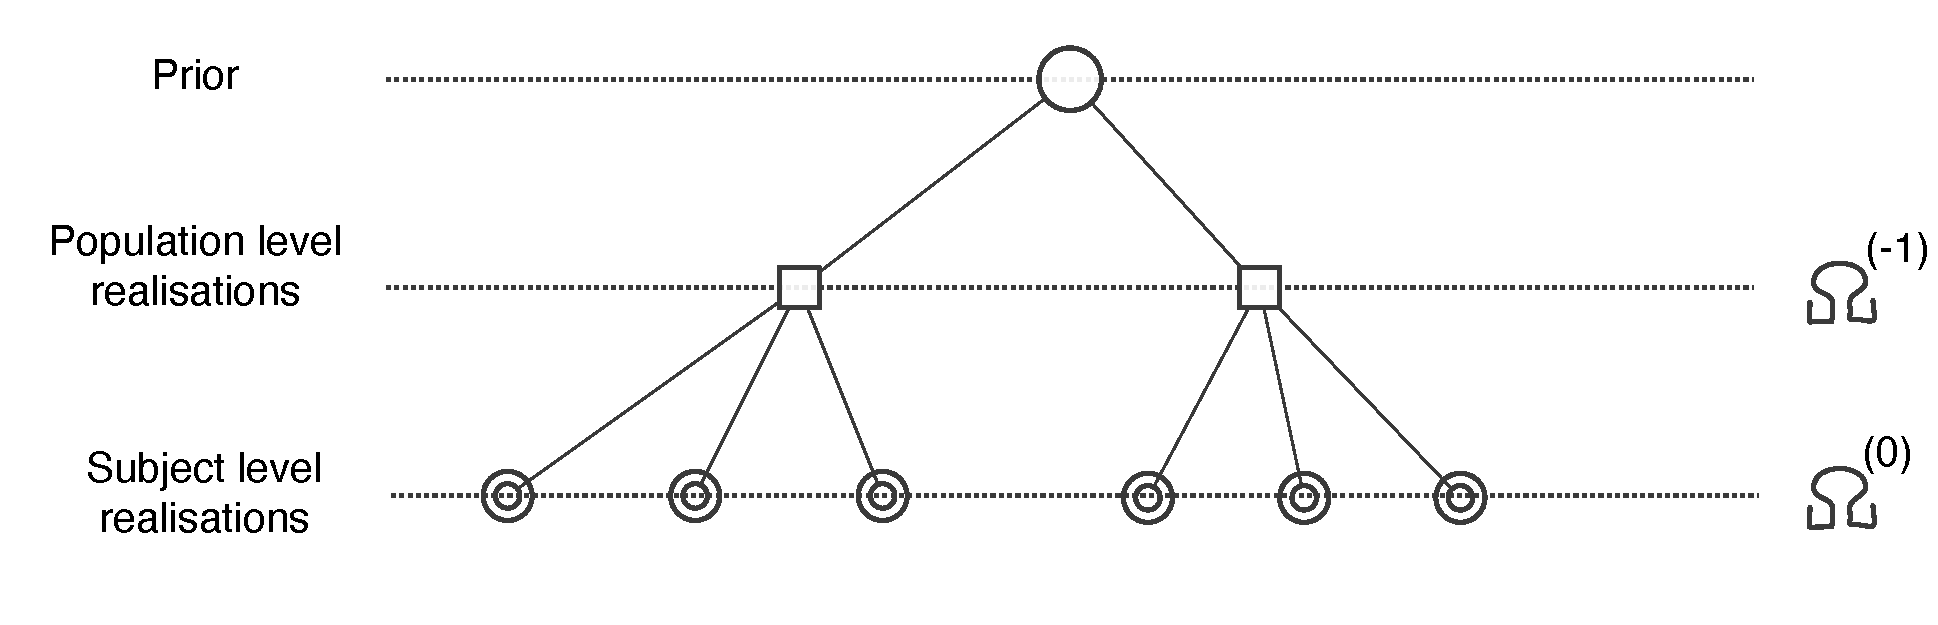
\includegraphics[width=140mm]{pics/IOV0-prior}
\end{tabular}
\caption{Basic variability structure with prior, population and subject levels.}
\label{fig:priorVM1}
\end{figure}

%\begin{figure}[htb!]
%\centering
%\begin{tabular}{cc}
% 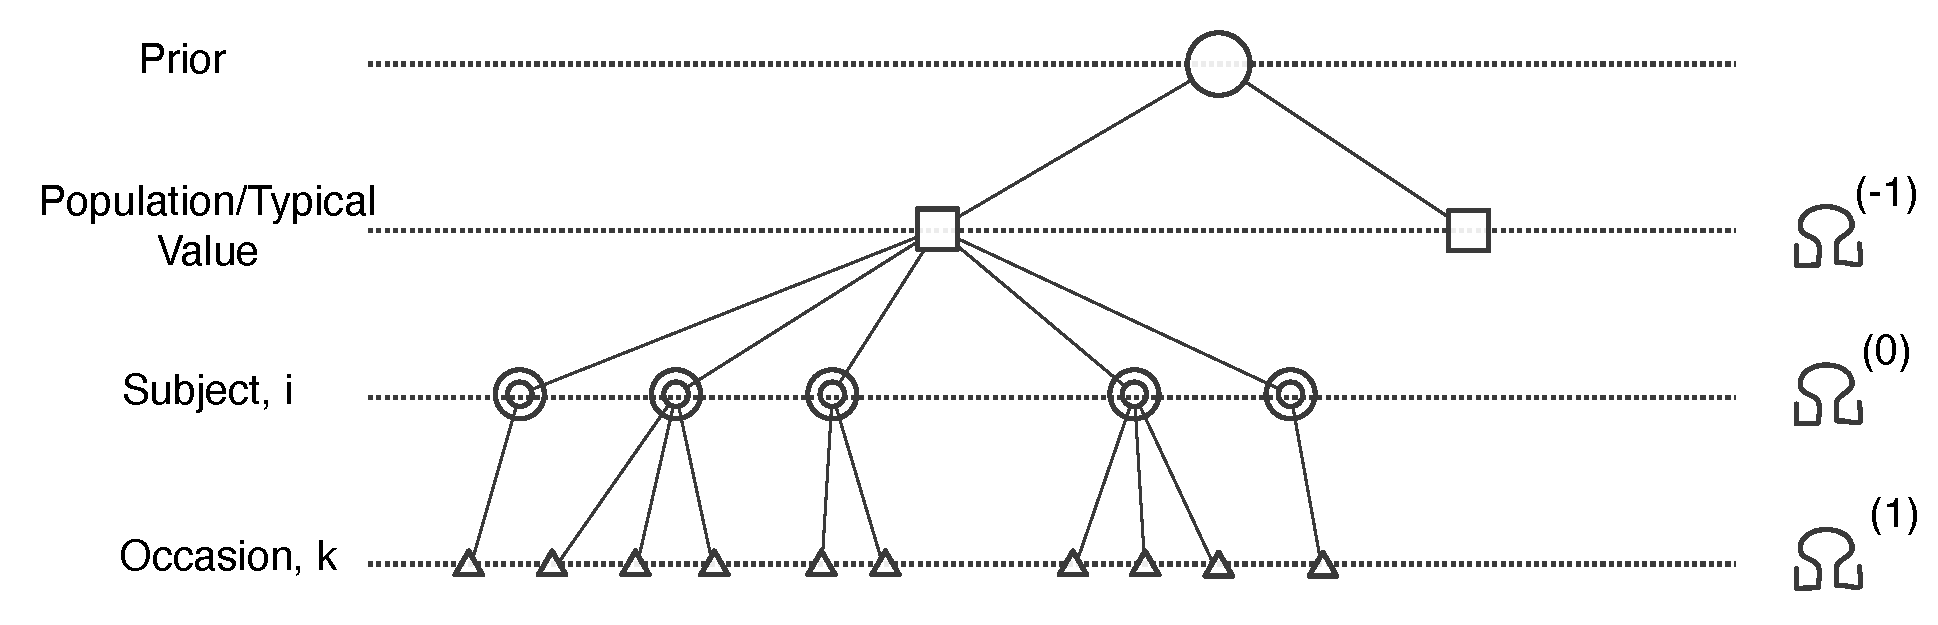
\includegraphics[width=140mm]{pics/IOV_2levels-prior}
%\end{tabular}
%\caption{Variability structure with IOV and priors on population parameters.}
%\label{fig:priorVM2}
%\end{figure}

In section \ref{sec:populationParameter} we have introduced the notation
for population parameters with associated prior distribution. In the following 
we discuss three complete examples, two estimation examples as formulated 
typically in winBUGS and a generic hierarchical model, which can be used
for simulation or estimation tasks.

\section{winBUGS \emph{Rats} example}
As an independent example, i.e. not directly related with pharmacometrics,  
we tested the schema with a use case from the winBUGS example collection, 
\cite{winBUGSvol1}.\\
The model
\begin{align*}
Y_{ij} &\sim \mathcal{N}(\alpha_i + \beta_i (x_j - x_{bar}), \tau_c) \\ 
\alpha_i &\sim \mathcal{N}(\alpha_c,\tau_{\alpha}) \\
\beta_i &\sim \mathcal{N}(\beta_c,\tau_{\beta}) 
\end{align*}
reads in winBUGS code
\lstset{language=MLX}
\begin{lstlisting}
		for( i in 1 : N ) {
			for( j in 1 : T ) {
				Y[i , j] ~ dnorm(mu[i , j],tau.c)
				mu[i , j] <- alpha[i] + beta[i] * (x[j] - xbar)
			}
			alpha[i] ~ dnorm(alpha.c,alpha.tau)
			beta[i] ~ dnorm(beta.c,beta.tau)
		} 
		tau.c~dgamma(0.001,0.001)
		alpha.c ~ dnorm(0.0,1.0E-6)
		alpha.tau ~ dgamma(0.001,0.001)
		beta.c ~ dnorm(0.0,1.0E-6)
		beta.tau ~ dgamma(0.001,0.001)
\end{lstlisting} 
\subparagraph{Observation model} is encoded using the previously introduced 
distribution type, \emph{O3}, section \ref{subsec:contModels}
\lstset{language=XML}
\begin{lstlisting}
        <ObservationModel blkId="om1">
            <ContinuousData>
                <General symbId="Y">
                    <ct:VariabilityReference>
                        <ct:SymbRef blkIdRef="vm2" symbIdRef="residual"/>
                    </ct:VariabilityReference>
                    <Distribution>
                        <ProbOnto name="Normal3">
                            <Parameter name="mean">
                                <ct:Assign>
                                    <ct:SymbRef blkIdRef="pm1" symbIdRef="mu"/>
                                </ct:Assign>
                            </Parameter>
                            <Parameter name="precision">
                                <ct:Assign>
                                    <ct:SymbRef blkIdRef="pm1" symbIdRef="tau.c"/>
                                </ct:Assign>
                            </Parameter>
                        </ProbOnto>
                    </Distribution>
                </General>
            </ContinuousData>
        </ObservationModel>
\end{lstlisting}
with the mean, $\mu$, and another two individual parameters, $\alpha$ and 
$\beta$ encoded next.
\subparagraph{Parameter model} We show only implementation for $\mu$ and $\alpha$ 
($\beta$ is encoded similarily). $\mu$ is an expression but it could have been
implemented directly in the observation model declaration making use of ProbOnto's capability
to assign any expressions to parameters.
\lstset{language=XML}
\begin{lstlisting}
        <IndividualParameter symbId="mu">
            <ct:Assign>
                <Equation xmlns="http://www.pharmml.org/pharmml/0.6/Maths">
                    <Binop op="plus">
                        <ct:SymbRef symbIdRef="alpha"/>
                        <Binop op="times">
                            <ct:SymbRef symbIdRef="beta"/>
                            <Binop op="minus">
                                <ct:SymbRef symbIdRef="x"/>
                                <ct:SymbRef symbIdRef="xbar"/>
                            </Binop>
                        </Binop>
                    </Binop>
                </Equation>
            </ct:Assign>
        </IndividualParameter>
\end{lstlisting}.

\lstset{language=XML}
\begin{lstlisting}
        <IndividualParameter symbId="alpha">
            <ct:VariabilityReference>
                <ct:SymbRef blkIdRef="vm1" symbIdRef="subject"/>
            </ct:VariabilityReference>
            <Distribution>
                <ProbOnto name="Normal3">
                    <Parameter name="mean">
                        <ct:Assign>
                            <ct:SymbRef symbIdRef="alpha.c"/>
                        </ct:Assign>
                    </Parameter>
                    <Parameter name="precision">
                        <ct:Assign>
                            <ct:SymbRef symbIdRef="alpha.tau"/>
                        </ct:Assign>
                    </Parameter>
                </ProbOnto>
            </Distribution>
        </IndividualParameter>
\end{lstlisting}
\subparagraph{Priors} All remaining population parameters $\tau_c$, $\alpha_c$, 
$\alpha_{\tau}$, $\beta_c$, $\beta_{\tau}$ are given \emph{non-informative} 
priors (using Normal or Gamma distribution) and for simplicity we show only the first two.
\lstset{language=XML}
\begin{lstlisting}
        <PopulationParameter symbId="tau.c">
            <ct:VariabilityReference>
                <ct:SymbRef blkIdRef="vm1" symbIdRef="pop"/>
            </ct:VariabilityReference>
            <Distribution>
                <ProbOnto name="Gamma">
                    <Parameter name="shape">
                        <ct:Assign>
                            <ct:Real>0.001</ct:Real>
                        </ct:Assign>
                    </Parameter>
                    <Parameter name="scale">
                        <ct:Assign>
                            <ct:Real>0.001</ct:Real>
                        </ct:Assign>
                    </Parameter>
                </ProbOnto>
            </Distribution>
        </PopulationParameter>
        
        <PopulationParameter symbId="alpha.c">
            <ct:VariabilityReference>
                <ct:SymbRef blkIdRef="vm1" symbIdRef="pop"/>
            </ct:VariabilityReference>
            <Distribution>
                <ProbOnto name="Normal3">
                    <Parameter name="mean">
                        <ct:Assign>
                            <ct:Real>0.0</ct:Real>
                        </ct:Assign>
                    </Parameter>
                    <Parameter name="precision">
                        <ct:Assign>
                            <ct:Real>1.0E-6</ct:Real>
                        </ct:Assign>
                    </Parameter>
                </ProbOnto>
            </Distribution>
        </PopulationParameter>
\end{lstlisting}

\section{PK example}

This example, based on the section 3.3.2 in \cite{Chiudinelli2015}, comes with correlated
parameters V, k and Vpop, kpop. Here the original model description is used: 
\emph{In this case, the model parameters are not independent random variables 
at both the individual and population level.} It will be useful to present few new 
features such as
\begin{itemize}
\item 
multivariate distributions with parameters, e.g. $\mathcal {MVN}$
\begin{itemize}
\item 
mean as vector
\item 
covariance matrix 
\end{itemize}
\item 
matrix operators, e.g. inverse of a matrix
\item 
new distribution type, the gamma distribution $\Gamma (,)$
\end{itemize}

\subsection{Model definition}

\subparagraph{Parameter model}
\begin{align*}
\left(\begin{array}{c} \log(V_j) \\
\log(k_j) \end{array}\right) & \sim
\mathcal {MVN} \left( \Big(\begin{array}{c} \log(V_{pop}) \\ \log(k_{pop}) \end{array}\Big),\Omega_P \right)\\
\log(\tau_{e_j}) &\sim \mathcal N \big(\log(\tau_{pop}),\omega_{\tau}^2\big)
\end{align*}

\subparagraph{Prior distributions}
\begin{align*}
\left(\begin{array}{c} \log(V_{pop}) \\
\log(k_{pop}) \end{array}\right) & \sim
\mathcal {MVN} \left( \Big(\begin{array}{c} \log(\mu_{V_{pop}}) \\ \log(\mu_{k_{pop}}) \end{array}\Big),\Sigma_{P_{pop}} \right)\\
\Omega_P^{-1} &\sim \mathcal {W} (R^{-1},\rho)\\
\omega_{\tau}^{-2} &\sim \Gamma (a_{\omega_{\tau}^2},b_{\omega_{\tau}^2})\\
\tau_{pop} &\sim \Gamma (a_{\tau_{pop}},b_{\tau_{pop}})
\end{align*}

\subparagraph{Structural and observation models}
\begin{align*}
	z_{ij} &\sim \mathcal N(c_{ij},\sigma_{e_j}^2) \\
	c_{ij} &= D/V_j e^{-k_j t_i}
\end{align*}

\subsection{Model implementation}
We will skip the structural and observation models as they don't contribute
any new insights in the discussion relevant to this chapter. Otherwise, we follow 
the winBUGS code as provided, with few following changes 
\begin{itemize}
\item 
removed \xelem{RandomVariable} declaration for \xatt{eps} because of the 
usage of distribution type observation model as defined in the model. 
Accordingly \xelem{Standard} has been replaced by \xelem{General} with 
\xelem{Distribution} tags (see \textit{Type O1}, \textit{Type O3} discussion 
in table \ref{tab:typeComparison}).
\end{itemize}


\paragraph{Parameter model} 
The individual parameters V and k have to be jointly extracted from a 
multivariate distribution. In particular, log(V) and log(k) are the elements 
of a vector, which is distributed as a multivariate normal with specific 
population mean and covariance matrix describing the inter-individual variability.

In the WinBUGS code, the multivariate normal requires the vector mean 
and the inverse of covariance matrix as arguments, while in PharmML it has 
been defined with vector mean and covariance matrix.
On the other hand, the individual parameter tau\_e is defined via a univariate 
normal distribution.

\lstset{language=MLX}
\begin{lstlisting}
	#correlated distribution of V and k of the j-subject
	lP[j,1:2]~dmnorm(lPpop[], TP[ , ])
\end{lstlisting}
in PharmML reads
\lstset{language=XML}
\begin{lstlisting}
            <PopulationParameter symbId="lP">
                <ct:VariabilityReference>
                    <ct:SymbRef symbIdRef="indiv" blkIdRef="model"/>
                </ct:VariabilityReference>
                <Distribution>
                    <ProbOnto name="MultivariateNormal1">
                        <Parameter name="mean">
                            <ct:Assign>
                                <ct:SymbRef symbIdRef="lPOP_P"/>
                            </ct:Assign>
                        </Parameter>
                        <Parameter name="covarianceMatrix">
                            <ct:Assign>
                                <ct:SymbRef symbIdRef="OMEGA_P"/>
                            </ct:Assign>
                        </Parameter>
                    </ProbOnto> 
                </Distribution>
            </PopulationParameter>
\end{lstlisting}
and
\lstset{language=MLX}
\begin{lstlisting}
	#distribution of taue of the j-subject
	ltaue[j]~dnorm(lTpop, Ttau)
	taue[j] <- exp(ltaue[j])
\end{lstlisting}
in PharmML reads
\lstset{language=XML}
\begin{lstlisting}
        <IndividualParameter symbId="TAU">
            <StructuredModel>
                <Transformation type="log"/>
                <LinearCovariate>
                    <PopulationValue>
                        <ct:Assign>
                            <ct:SymbRef symbIdRef="POP_T"/>
                        </ct:Assign>
                    </PopulationValue>
                </LinearCovariate>
                <RandomEffects>
                    <ct:SymbRef symbIdRef="eta_T"/>
                </RandomEffects>
            </StructuredModel>
        </IndividualParameter>
\end{lstlisting}
with implementation of \emph{eta\_T} not shown here as it uses the 
well known \xelem{RandomVariable} element for its encoding.\\
The V and k individual parameters have to be retrieved. The elements of the lP vector 
are log(V) and log(k), so the exponential of the lP elements must be computed to obtain V and k.

\lstset{language=MLX}
\begin{lstlisting}
	lV[j] <- lP[j,1]
	V[j] <- exp(lV[j]) 
	lk[j] <- lP[j,2]
	k[j] <- exp(lk[j]) 
\end{lstlisting}
in PharmML reads
\lstset{language=XML}
\begin{lstlisting}
        <IndividualParameter symbId="V">
            <ct:Assign>
                <Equation xmlns="http://www.pharmml.org/pharmml/0.6/Maths">
                    <Uniop op="exp">
                        <ct:VectorSelector>
                            <ct:SymbRef symbIdRef="lP"/>
                            <ct:Cell>
                                <ct:Int>2</ct:Int>
                            </ct:Cell>
                        </ct:VectorSelector>
                    </Uniop>
                </Equation>
            </ct:Assign>
        </IndividualParameter>
        
        <!-- k omitted here -->
\end{lstlisting}

\paragraph{Priors} specification  \\
The prior model on the fixed effect 'tau\_Ppop' reads
\lstset{language=MLX}
\begin{lstlisting}
	# prior on "THETA"
	tau_Ppop[1:2, 1:2] <- inverse(sigma_Ppop[ , ])
\end{lstlisting}
and requires the definition of the matrix and it reads in PharmML as
\lstset{language=XML}
\begin{lstlisting}
            <PopulationParameter symbId="SIGMA_POP_P">
                <ct:Assign>
                    <ct:Matrix matrixType="Any">
                        <ct:MatrixRow>
                            <ct:RowIndex><ct:Int>1</ct:Int></ct:RowIndex>
                            <ct:Real>1</ct:Real>
                            <ct:Real>0.1</ct:Real>
                            </ct:MatrixRow>
                        <ct:MatrixRow>
                            <ct:RowIndex><ct:Int>2</ct:Int></ct:RowIndex>
                            <ct:Real>0.1</ct:Real>
                            <ct:Real>1</ct:Real>
                        </ct:MatrixRow>
                    </ct:Matrix>
                </ct:Assign>
            </PopulationParameter>
\end{lstlisting}
The vector of the population values
\lstset{language=MLX}
\begin{lstlisting}
	lmu_Ppop[1] <- log(mu_Vpop)
	lmu_Ppop[2] <- log(mu_kpop)
\end{lstlisting}
reads in PharmML 
\lstset{language=XML}
\begin{lstlisting}
        <PopulationParameter symbId="lMU_POP_P">
            <ct:Assign>
                <ct:Vector>
                    <ct:VectorElements>
                        <ct:SymbRef symbIdRef="lMU_POP_K"/>
                        <ct:SymbRef symbIdRef="lMU_POP_V"/>
                    </ct:VectorElements>
                </ct:Vector>
            </ct:Assign>
        </PopulationParameter>
        
        <PopulationParameter symbId="lMU_POP_V">
            <ct:Assign>
                <Equation xmlns="http://www.pharmml.org/pharmml/0.6/Maths">
                    <Uniop op="log">
                        <ct:SymbRef symbIdRef="MU_POP_V"/>
                    </Uniop>
                </Equation>
            </ct:Assign>
        </PopulationParameter>
        <!-- with -->        
        <PopulationParameter symbId="MU_POP_V"/>
        <!-- k omitted here -->
\end{lstlisting}
The vector of log of the population parameters Vpop and kpop is a-priori distributed as a multivariate Normal with user-defined vector mean and covariance matrix, reported above.
\lstset{language=MLX}
\begin{lstlisting}
	lPpop[1:2]~dmnorm(lmu_Ppop[], tau_Ppop[ , ])
\end{lstlisting}
reads in PharmML 
\lstset{language=XML}
\begin{lstlisting}
        <PopulationParameter symbId="lPOP_P">
            <ct:VariabilityReference>
                <ct:SymbRef symbIdRef="pop" blkIdRef="model"/>
            </ct:VariabilityReference>
            <Distribution>
                <ProbOnto name="MultivariateNormal1">
                    <Parameter name="mean">
                        <ct:Assign>
                            <ct:SymbRef symbIdRef="lMU_POP_P"/>
                        </ct:Assign>
                    </Parameter>
                    <Parameter name="covarianceMatrix">
                        <ct:Assign>
                            <ct:SymbRef symbIdRef="SIGMA_POP_P"/>
                        </ct:Assign>
                    </Parameter>
                </ProbOnto>
            </Distribution>
        </PopulationParameter>
\end{lstlisting}
with the according covariance matrix \emph{SIGMA\_POP\_P} defined above.

The inverse of the covariance matrix \emph{OMEGA\_P} is distributed as a Wishart with given parameters R and rho (not reported). A different parametrization has been used in WinBUGS (in which the inverse of R is required) and PharmML (in which the Wishart1 distribution enables the use of the R matrix)
\lstset{language=MLX}
\begin{lstlisting}
	# prior on inverse of "OMEGA"
	Rinv[1:2,1:2] <- inverse(R[,])
	TP[1:2,1:2]~dwish(Rinv[ , ], rho)
\end{lstlisting}
in PharmML reads
\lstset{language=XML}
\begin{lstlisting}
        <PopulationParameter symbId="OMEGA_P">
            <ct:Assign>
                <Equation xmlns="http://www.pharmml.org/pharmml/0.6/Maths">
                    <MatrixUniop op="inverse">
                        <ct:SymbRef symbIdRef="invOMEGA_P"/>
                    </MatrixUniop>
                </Equation>
            </ct:Assign>
        </PopulationParameter>
        
        <PopulationParameter symbId="invOMEGA_P">
            <ct:VariabilityReference>
                <ct:SymbRef symbIdRef="pop" blkIdRef="model"/>
            </ct:VariabilityReference>
            <Distribution>
                <ProbOnto name="Wishart1">
                    <Parameter name="scaleMatrix">
                        <ct:Assign>
                            <ct:SymbRef symbIdRef="rho"/>
                        </ct:Assign>
                    </Parameter>
                    <Parameter name="degreesOfFreedom">
                        <ct:Assign>
                            <ct:SymbRef symbIdRef="R"/>
                        </ct:Assign>
                    </Parameter>
                </ProbOnto>
            </Distribution>
        </PopulationParameter>
\end{lstlisting}
The inverse of the variance of \emph{eta\_T} (\emph{OMEGA\_T}) is a-priori distributed as a Gamma with user-defined parameters.
\lstset{language=MLX}
\begin{lstlisting}
	Ttau~dgamma(a_omega_tau, b_omega_tau)
\end{lstlisting}
in PharmML reads
\lstset{language=XML}
\begin{lstlisting}
        <PopulationParameter symbId="TAU_T">
            <ct:VariabilityReference>
                <ct:SymbRef symbIdRef="pop" blkIdRef="model"/>
            </ct:VariabilityReference>
            <Distribution>
                <ProbOnto name="Gamma">
                    <Parameter name="shape">
                        <ct:Assign>
                            <ct:SymbRef symbIdRef="a_OMEGA_T"/>
                        </ct:Assign>
                    </Parameter>
                    <Parameter name="scale">
                        <ct:Assign>
                            <ct:SymbRef symbIdRef="b_OMEGA_T"/>
                        </ct:Assign>
                    </Parameter>
                </ProbOnto>
            </Distribution>
        </PopulationParameter>
        
        <PopulationParameter symbId="OMEGA_T">
            <ct:Assign>
                <Equation xmlns="http://www.pharmml.org/pharmml/0.6/Maths">
                    <Binop op="divide">
                        <ct:Real>1</ct:Real>
                        <ct:SymbRef symbIdRef="TAU_T"/>
                    </Binop>
                </Equation>
            </ct:Assign>
        </PopulationParameter>
\end{lstlisting}
\emph{POP\_T} is a-priori distributed as a Gamma with user-defined parameters.
\lstset{language=MLX}
\begin{lstlisting}
	# prior on "SIGMA"
	Tpop~dgamma(a_taupop, b_taupop)
	lTpop <- log(Tpop)
\end{lstlisting}
in PharmML reads
\lstset{language=XML}
\begin{lstlisting}
        <PopulationParameter symbId="POP_T">
            <ct:VariabilityReference>
                <ct:SymbRef symbIdRef="pop" blkIdRef="model"/>
            </ct:VariabilityReference>
            <Distribution>
                <ProbOnto name="Gamma">
                    <Parameter name="shape">
                        <ct:Assign>
                            <ct:SymbRef symbIdRef="a_POP_T"/>
                        </ct:Assign>
                    </Parameter>
                    <Parameter name="scale">
                        <ct:Assign>
                            <ct:SymbRef symbIdRef="b_POP_T"/>
                        </ct:Assign>
                    </Parameter>
                </ProbOnto>
            </Distribution>
        </PopulationParameter>
\end{lstlisting}



The structural model is a standard algebraic equations and its implementation
will not be shown here. The Observation model on the other hand is implemented
using the distribution model and read in PharmML:
\lstset{language=XML}
\begin{lstlisting}
        <General symbId="C">
            <ct:VariabilityReference>
                <ct:SymbRef blkIdRef="resErrorModel" symbIdRef="residual"/>
            </ct:VariabilityReference>
            <Distribution>
                <ProbOnto name="Normal2">
                    <Parameter name="mean">
                        <ct:Assign>
                            <ct:SymbRef blkIdRef="sm1" symbIdRef="C"/>
                        </ct:Assign>
                    </Parameter>
                    <Parameter name="var">
                        <ct:Assign>
                            <ct:SymbRef symbIdRef="sigmaSquare"/>
                        </ct:Assign>
                    </Parameter>
                </ProbOnto>
            </Distribution>
        </General>
\end{lstlisting}
with
\lstset{language=XML}
\begin{lstlisting}
        <IndividualParameter symbId="sigmaSquare">
            <ct:Assign>
                <Equation xmlns="http://www.pharmml.org/pharmml/0.6/Maths">
                    <Uniop op="sqrt">
                        <Binop op="divide">
                            <ct:Real>1</ct:Real>
                            <ct:SymbRef symbIdRef="TAU"/>
                        </Binop>
                    </Uniop>
                </Equation>
            </ct:Assign>
        </IndividualParameter>
\end{lstlisting}
declared in parameter model, \xatt{pm1}.

\section{Hierarchical model example}
The following model has been proposed by Marc Lavielle, \cite{LavielleFourModels:2014},
to test the capabilities of the DDMoRe platform with respect to the encoding of
hierarchical models, encoded here in MLXTRAN
\lstset{language=MLX}
\begin{lstlisting}
    [LONGITUDINAL]
    input = {V, k, b}
    EQUATION:
    D=100
    f = D/V*exp(-k*t)
    DEFINITION:
    y = {distribution=normal, prediction=f, sd=b*f}

    [INDIVIDUAL]
    input = {V_pop, omega_V, w, w_pop}
    EQUATION:
    V_pred = V_pop*(w/w_pop)
    DEFINITION:
    V = {distribution=logNormal, prediction=V_pred, sd=omega_V}

    [COVARIATE]
    input = {w_pop, omega_w}
    DEFINITION:
    w = {distribution=normal, mean=w_pop, sd=omega_w}

    [POPULATION]
    input = {ws, gw, Vs, gV}
    DEFINITION:
    w_pop = {distribution=normal, mean=ws, sd=gw}
    V_pop = {distribution=logNormal, mean=log(Vs), sd=gV}
\end{lstlisting}
In the following we will show only the relevant for this chapter model elements.
\paragraph{Observation model}
\begin{align*}
 y \sim \mathcal N(f,b f)
\end{align*}
reads in PharmML
\lstset{language=XML}
\begin{lstlisting}
    <General symbId="y">
        <ct:VariabilityReference>
            <ct:SymbRef blkIdRef="vm2" symbIdRef="resErr"/>
        </ct:VariabilityReference>
        <Distribution>
            <ProbOnto name="Normal1">
                <Parameter name="mean">
                    <ct:Assign>
                        <ct:SymbRef blkIdRef="sm1" symbIdRef="f"/>
                    </ct:Assign>
                </Parameter>
                <Parameter name="stdev">
                    <ct:Assign>
                        <math:Equation>
                            <math:Binop op="times">
                                <ct:SymbRef blkIdRef="pm1" symbIdRef="b"/>
                                <ct:SymbRef blkIdRef="sm1" symbIdRef="f"/>
                            </math:Binop>
                        </math:Equation>
                    </ct:Assign>
                </Parameter>
            </ProbOnto>
        </Distribution>
    </General>
\end{lstlisting}
Note the encoding of expressions in the second parameter of the normal distribution
easily done when using ProbOnto, was not possible with UncertML.
\paragraph{Individual parameter model} 
\begin{align*}
 V \sim \mathcal {LN}(V_{pred}, \omega_V) \quad \text{with} \quad V_{pred}=V_{pop} (w/w_{pop})
\end{align*}
reads in PharmML:
\lstset{language=XML}
\begin{lstlisting}
    <IndividualParameter symbId="V">
        <ct:VariabilityReference>
            <ct:SymbRef blkIdRef="vm1" symbIdRef="indiv"/>
        </ct:VariabilityReference>
        <Distribution>
            <ProbOnto name="LogNormal1">
                <Parameter name="meanLog">
                    <ct:Assign>
                        <ct:SymbRef symbIdRef="V_pred"/>
                    </ct:Assign>
                </Parameter>
                <Parameter name="stdevLog">
                    <ct:Assign>
                        <ct:SymbRef symbIdRef="omega_V"/>
                    </ct:Assign>
                </Parameter>
            </ProbOnto>
        </Distribution>
    </IndividualParameter>

    <!-- V_pred = V_pop*(w/w_pop) -->
    <PopulationParameter symbId="V_pred">
        <ct:Assign>
            <math:Equation>
                <math:Binop op="times">
                    <ct:SymbRef symbIdRef="V_pop"/>
                    <math:Binop op="divide">
                        <ct:SymbRef blkIdRef="cm1" symbIdRef="w"/>
                        <ct:SymbRef symbIdRef="w_pop"/>
                    </math:Binop>
                </math:Binop>
            </math:Equation>
        </ct:Assign>
    </PopulationParameter>
\end{lstlisting}
\paragraph{Covariate model} describes the distribution of body weight
\begin{align*}
 w \sim \mathcal {N}(w_{pop}, \omega_w)
\end{align*}
can be encoded as
\lstset{language=XML}
\begin{lstlisting}
    <CovariateModel blkId="cm1">
        <Covariate symbId="w">
            <Continuous>
                <Distribution>
                    <ProbOnto name="Normal1">
                        <Parameter name="mean">
                            <ct:Assign>
                                <ct:SymbRef blkIdRef="pm1" symbIdRef="w_pop"/>
                            </ct:Assign>
                        </Parameter>
                        <Parameter name="stdev">
                            <ct:Assign>
                                <ct:SymbRef blkIdRef="pm1" symbIdRef="omega_w"/>
                            </ct:Assign>
                        </Parameter>
                    </ProbOnto>
                </Distribution>
            </Continuous>
        </Covariate>
    </CovariateModel>
\end{lstlisting}
Note, that the population parameters used in the covariate model are 
defined in the parameter model, \xatt{pm1}, as the next code snippet will show.
\paragraph{Population parameters} of the model covariate model 
\begin{align*}
 w_{pop} \sim \mathcal {N}(ws, gw)
\end{align*}
and
\begin{align*}
 V_{pop} \sim \mathcal {LN}\big(\log(V\!s), gV\big)
\end{align*}
are encode as
\lstset{language=XML}
\begin{lstlisting}
    <!-- w_pop = {distribution=normal, mean=ws, sd=gw} -->
    <PopulationParameter symbId="w_pop">
        <ct:VariabilityReference>
            <ct:SymbRef blkIdRef="vm1" symbIdRef="pop"/>
        </ct:VariabilityReference>
        <Distribution>
            <ProbOnto name="Normal1">
                <Parameter name="mean">
                    <ct:Assign>
                        <ct:SymbRef symbIdRef="ws"/>
                    </ct:Assign>
                </Parameter>
                <Parameter name="stdev">
                    <ct:Assign>
                        <ct:SymbRef symbIdRef="gw"/>
                    </ct:Assign>
                </Parameter>
            </ProbOnto>
        </Distribution>
    </PopulationParameter>

    <!-- V_pop = {distribution=logNormal, mean=log(Vs), sd=gV} -->
    <PopulationParameter symbId="V_pop">
        <ct:VariabilityReference>
            <ct:SymbRef blkIdRef="vm1" symbIdRef="pop"/>
        </ct:VariabilityReference>
        <Distribution>
            <ProbOnto name="LogNormal1">
                <Parameter name="meanLog">
                    <ct:Assign>
                        <math:Equation>
                            <math:Uniop op="log">
                                <ct:SymbRef symbIdRef="Vs"/>
                            </math:Uniop>
                        </math:Equation>
                    </ct:Assign>
                </Parameter>
                <Parameter name="stdevLog">
                    <ct:Assign>
                        <ct:SymbRef symbIdRef="gV"/>
                    </ct:Assign>
                </Parameter>
            </ProbOnto>
        </Distribution>
    </PopulationParameter>
\end{lstlisting}


%%%%%%%%%%%%%%%%%%%%%%%%%%%%%%%%%%%%%%%%%%%%%%%%%%%%%%%%%%%%%%%%%%%%%%
\section{Additional examples implemented}
In addition eight examples as described in \cite{Chiudinelli2015} have been 
successfully implemented in PharmML 0.7 and are provided with the release:
\emph{example331.xml}, \emph{example332.xml}, \emph{example333.xml}, 
\emph{example334.xml}, \emph{example335.xml}, \emph{example3311.xml},
\emph{example3312.xml}, \emph{example3321.xml}.




%%%%%%%%%%%%%%%%%%%%%%%%%%%%%%%%%%%%%%%%%%%%%%%%%%%%%%%%%%%%%%%%%%%%%%
%%%%%%%%%%%%%%%%%%%%%%%%%%%%%%%%%%%%%%%%%%%%%%%%%%%%%%%%%%%%%%%%%%%%%%%
%%%%%%%%%%%%%%%%%%%%%%%%%%%%%%%%%%%%%%%%%%%%%%%%%%%%%%%%%%%%%%%%%%%%%%%
%%%%%%%%%%%%%%%%%%%%%%%%%%%%%%%%%%%%%%%%%%%%%%%%%%%%%%%%%%%%%%%%%%%%%%%
\chapter{Design -- redesigned}
\label{ch:Design}

%%%%%%%%%%%%%%%%%%%%%%%%%%%%%%%%%%%%%%%%%%%%%%%%%%%%%%%%%%%%%%%%%%%%%%
\section{Design in PharmML $\leq$ 0.6}
Since version 0.2 PharmML was using SDM-XML, a CDISC standard \cite{CDISC:2011a}, 
based trial design. With the beginning of the activities of a group working on trial design
for MDL it became clear that this structure is insufficient and had to be reorganised and 
redesigned, see figure \ref{fig:Flowchart07}. The main reasons are 
\begin{itemize}
\item
CDISC based design is missing many elements, the most important ones being 
the observations and design spaces. Although the former were supported in 
PharmML, their implementation not only had to be done in \xelem{ModellingSteps} 
section but it also lacked the connectivity to study arms.
\item
A number of typical design features, such as arm size, number of arms, total size,
number of samples, number of times, cost function, total cost, was not accounted for.
\item
The rigid structure with epochs/cells/segment was unfamiliar to modellers 
who need a more flexible arm based structure.
\item
Required specifically for optimal design, the re-definition of covariate 
model, required for covariates to be optimised, was not supported in the CDISC 
based structure.
\item
Design elements were spread over two sections, \xelem{TrialDesign} and \xelem{ModellingSteps}
which created an inconsistent structure.
\item
The specification of external datasets, was located in \xelem{ModellingSteps}, but as 
the source for design it belongs to trial design section.
\item
\xelem{ModellingSteps} section should contain only task description.
%- Separation between model-design-tasks required - in Steps only task description - with 2 new elements
\item
The lack of compatibility with the new MDL design proposal -- translation would be 
very hard to achieve given such two different structures.
\end{itemize}
The new design/trial design structure addresses the above issues and 
because it was developed with both MDL and PharmML in mind, it promises 
a very high \marginpar{\HandCuffLeft} degree of compatibility between 
these two languages -- to be verified during the coming months. 


%%%%%%%%%%%%%%%%%%%%%%%%%%%%%%%%%%%%%%%%%%%%%%%%%%%%%%%%%%%%%%%%%%%%%%
\section{Modifications and extensions}
The new trial design structure consists of
\begin{itemize}
\item
Core structure based on the design elements developed for MDL, \cite{Commets2015, CommetsExamples2015}.
\item
Additional features available in PharmML since 0.2.1 such as individual 
observations, dosing, covariates.
\end{itemize}
While the detailed design is described in the according MDL specification proposal, 
\cite{Commets2015}, the comparison on the following pages visualises the changes
and differences. In the left column on page \pageref{miniPage:comparison}, the PharmML 
$\leq$ 0.6 design elements are shown, distributed
over two sections, \xelem{TrialDesign} and \xelem{ModellingSteps}. 
On the right, a detailed list of current elements available for the trial design is given.

All examples provided in the 'Modelling Description Language. Design 
elements - Examples', \cite{CommetsExamples2015}, and all explicit design 
based examples from the PharmML specification, \cite{Pharmml_06}, have 
been successfully implemented.

\newpage
\begin{figure}[htb!]
\centering
  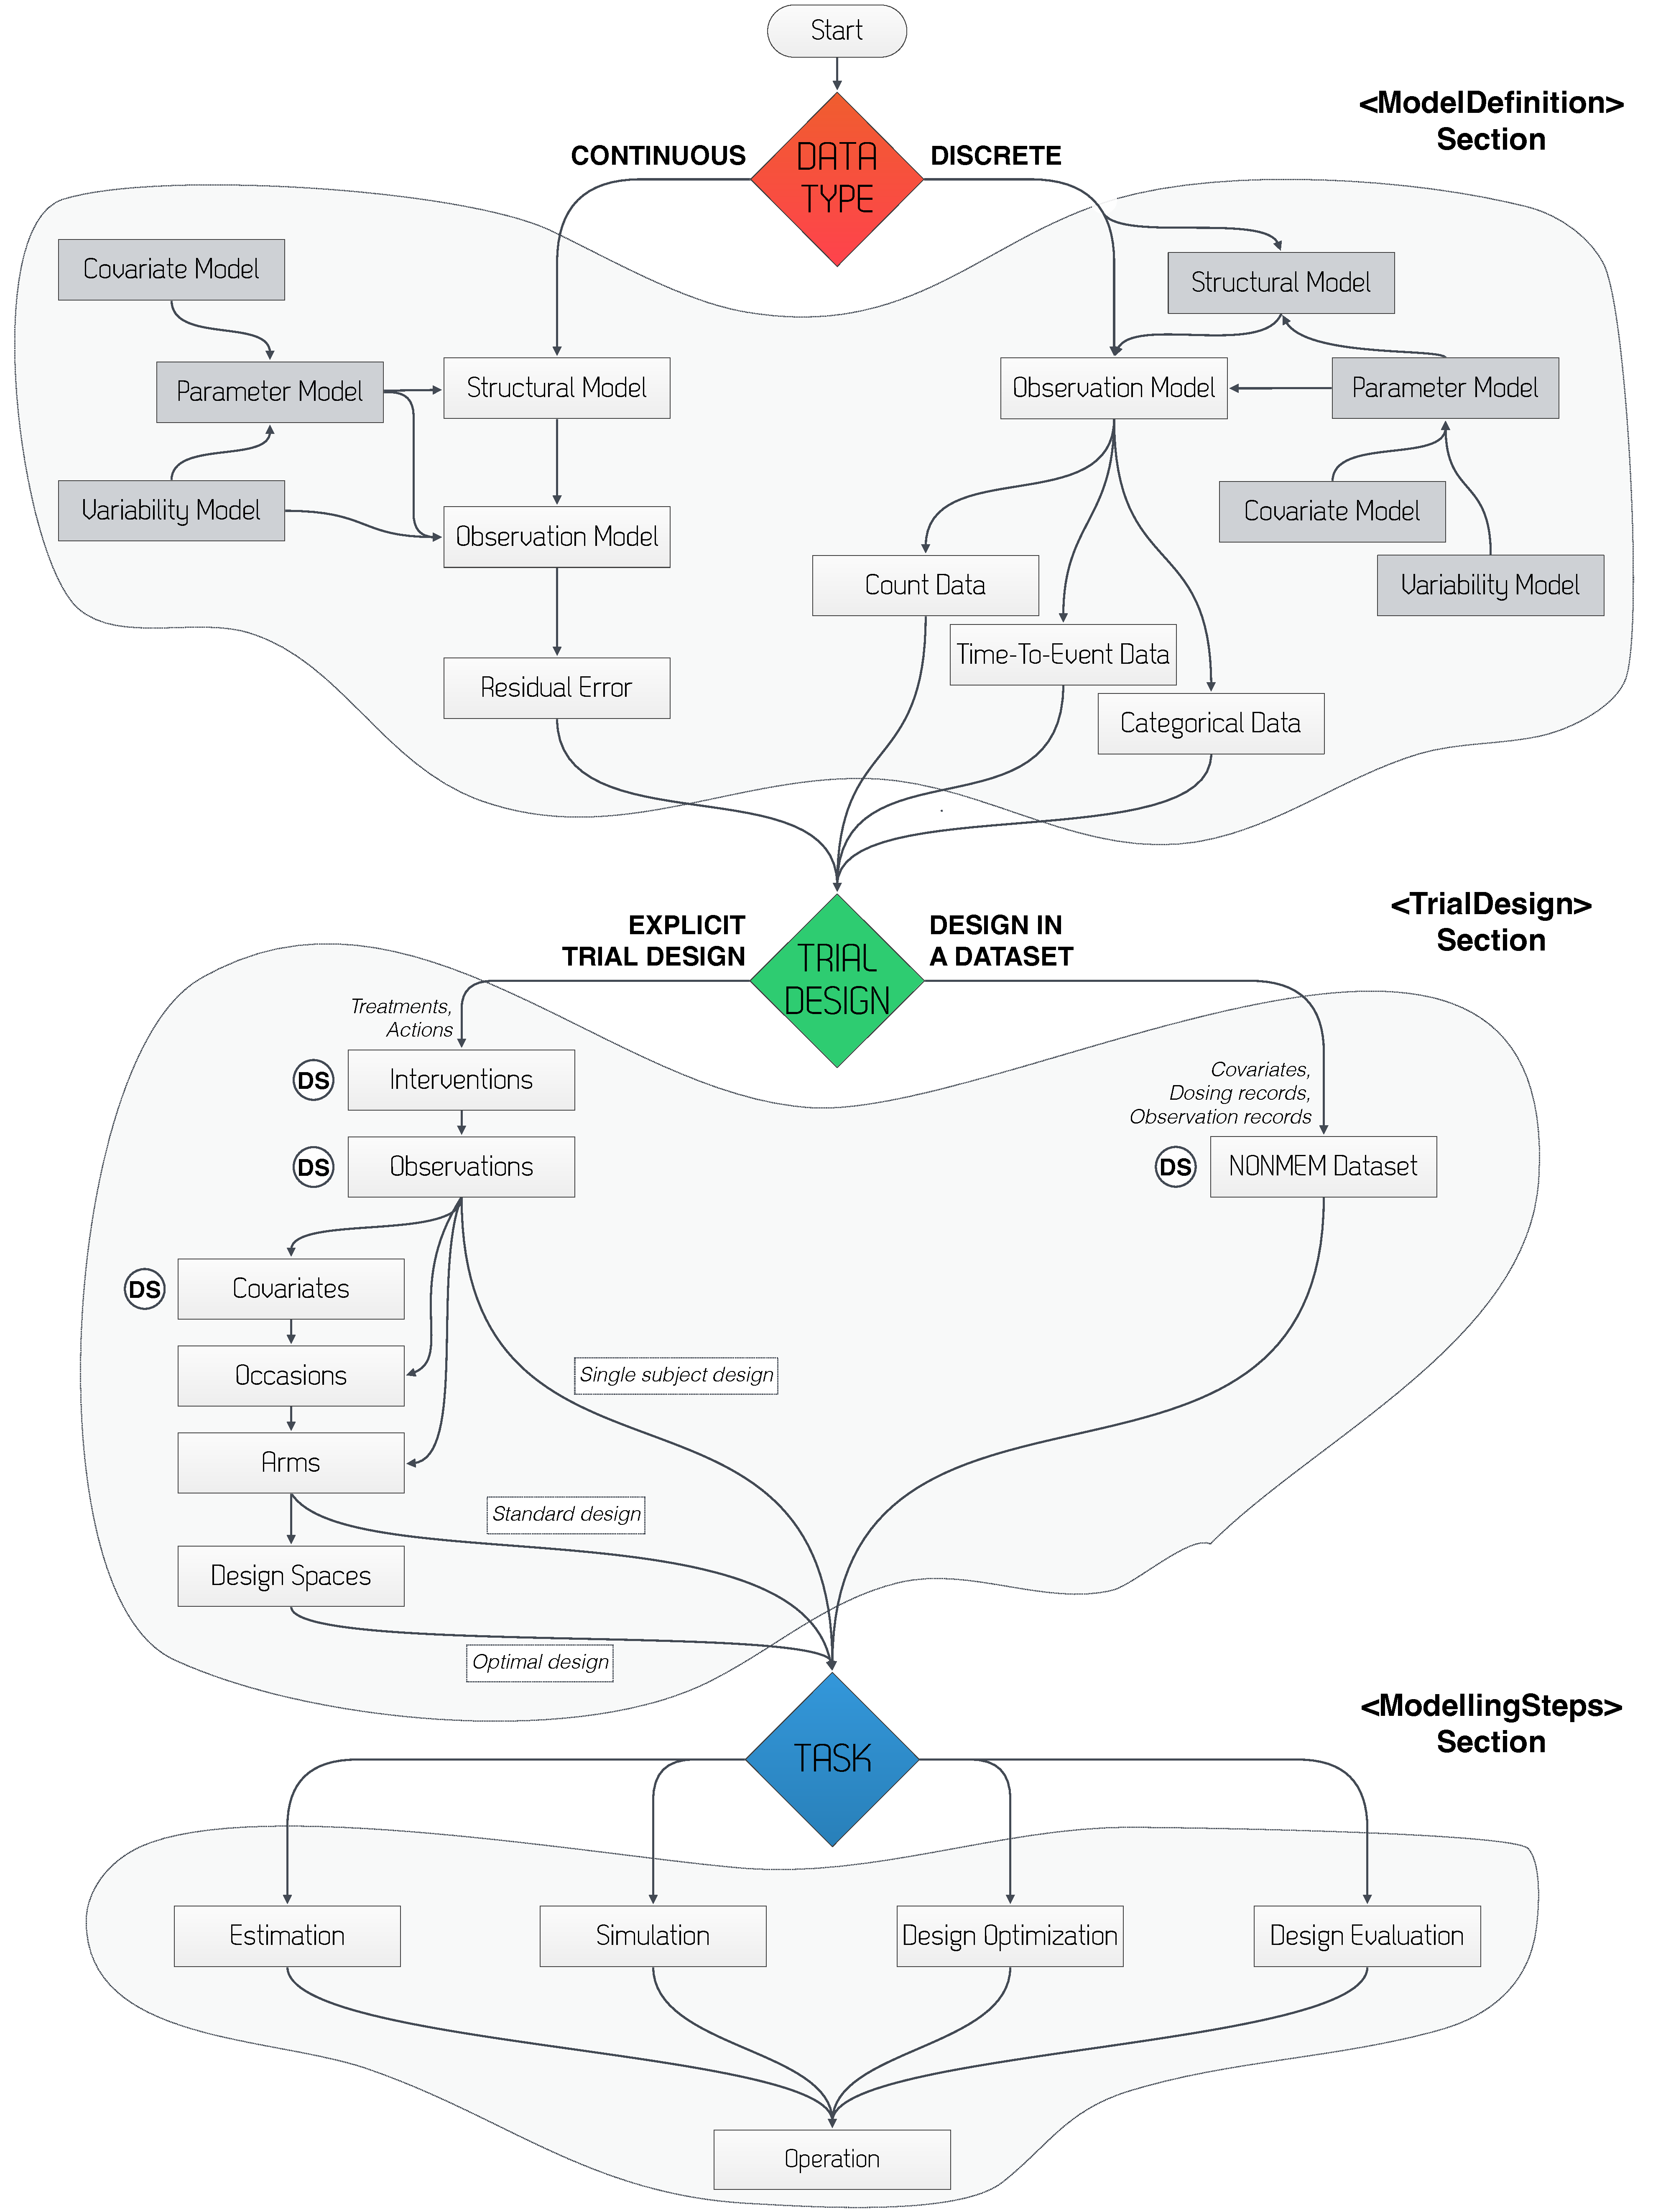
\includegraphics[width=165mm]{pics/Flowchart07}
 \caption{Working with PharmML -- a schema showing three essential decision points: 
 (A) the type of data (continuous and discrete), (B) the source of the study design and 
 data (Monolix/NONMEM dataset or \xelem{TrialDesign}) and finally (C) the task type 
 (for now only simulation and estimation tasks are fully supported, the design related 
 tasks are under construction). \textbf{Note} that in comparison to 0.6 version, \cite{Pharmml_06}, 
 all data and design elements are located in the \xelem{TrialDesign} section while the last 
 section, \xelem{ModellingSteps}, carries only tasks related information.}
 \label{fig:Flowchart07}
\end{figure}

\newpage

%\LTcapwidth=\textwidth
%\begin{center}
%\renewcommand{\arraystretch}{1.1}%
%\begin{longtable}{llcccc}
%  \hline
%  \hline
%0.6 & 0.7\\
%%\multicolumn{1}{c}{0.2}			& risation		&  3.0			& 1.4		& 4.3	& 7.3 \\
%  \hline
%
%  \hline \\
%\caption{Structure comparison of the trial design related features.}
%\label{Tab:NewOldDesign}
%%\vspace{-3.5em}
%\end{longtable}
%\end{center}


%%%%% LEFT PAGE %%%%%
\begin{minipage}{0.35\textwidth}
\small
\centering 
\pml $\le$ 0.6\\
{\color{red} \scshape{\xelem{TrialDesign}}}
\begin{flushleft} 
\begin{itemize}
\item 
Structure
\begin{itemize}
\item
Arm
\item
Cell
\item
Epoch
\item
Segment
\item
Activity
\begin{itemize}
\item
Bolus
\item
Infusion
\item
Washout
\item
Lookup table
\item
Epoch Ref/Period
\end{itemize}
\end{itemize}
\item
Population
\begin{itemize}
\item
Arm memberships \& covariates
\item
Demographics
\end{itemize}
\item 
Individual Dosing
\end{itemize}
\vspace{2em}
\end{flushleft}
\centering 
{\color{red} \scshape{\xelem{ModellingSteps}}}
\begin{flushleft} 
\begin{itemize}
\item 
\textbf{ExternalDataSet}
\item 
Simulation Step
\begin{itemize}
\item 
\textbf{Observations}
\item 
Operation
\end{itemize}
\item 
Estimation Step
\begin{itemize}
\item 
\textbf{ObjectiveData}
\item 
Parameter Estimation
\item 
Operation
\end{itemize}
\item 
Step dependencies
\end{itemize}
\end{flushleft}
\end{minipage}
%%%%% RIGHT PAGE %%%%%
\begin{minipage}{0.6\textwidth}
\small
\centering 
\pml 0.7\\
{\color{red} \scshape{\xelem{TrialDesign}}}
\begin{flushright}
\begin{itemize}
\item 
ExternalDataSet
\item 
Interventions
\begin{itemize}
\item 
Administration
\begin{itemize}
\item 
InterventionRef
\item
Bolus
\item
Infusion
\end{itemize}
\item 
IndividualAdministration
\item 
Action -- Washout
\begin{itemize}
\item 
full reset
\item 
variable-wise
\end{itemize}
\item
InterventionsCombination
\end{itemize}
\item 
Observations
\begin{itemize}
\item 
LookupTable 
\item 
IndividualObservations
\item 
Observation
\item 
ObservationsCombination
\end{itemize}
\item 
Covariates
\begin{itemize}
\item 
CovariateModel
\begin{itemize}
\item
Categorical/Category: Probability, OccasionRef, InterventionRef, InterventionSequence
\end{itemize}
\item 
IndividualCovariates
\end{itemize}
\item 
Occasions/OccasionList
\begin{itemize}
\item 
VariabilityReference
\item 
Occasion
\end{itemize}
\item 
Arms
\begin{itemize}
\item 
Simple elements: ArmSize, CostFunction, NumberArms, NumberSamples, NumberTimes, SameTimes, TotalCost, TotalSize
\item 
Arm
\begin{itemize}
\item 
Simple elements: ArmSize, NumberSamples, NumberTimes, SameTimes
\item 
InterventionSequence/List
\item 
ObservationSequence/List
\item 
OccasionSequence/List
\end{itemize}
\end{itemize}
\item 
DesignSpaces
\begin{itemize}
\item 
References: InterventionRef, ObservationRef, ArmRef, SymbRef, CovariateModelRef \& CovariateRef
\item 
Simple elements: ArmSize, DoseAmount, DosingTimes, Duration, NumberArms, NumberSamples, NumberTimes, SampleTimes
\end{itemize}
\end{itemize}
\end{flushright}
{\color{red} \scshape{\xelem{ModellingSteps}}}
\begin{flushleft} 
\begin{itemize}
\item 
Simulation Step w. Operation
\item 
Estimation Step w. Parameter Estimation \& Operation
\item 
Design Optimization Step -- {\color{darkgreen} \scshape{under construction}} 
\item 
Design Evaluation Step -- {\color{darkgreen} \scshape{under construction}}
\item 
Step dependencies
\end{itemize}
\end{flushleft}
\label{miniPage:comparison}
\end{minipage}



%%%%%%%%%%%%%%%%%%%%%%%%%%%%%%%%%%%%%%%%%%%%%%%%%%%%%%%%%%%%%%%%%%%%%%
\section{Selected features}
The trial design structure, although intuitive and relatively easy to learn,
is quite complex. The reader is referred to the original specification 
and example documents, \cite{CommetsExamples2015,Commets2015}.
Here we show only few examples of selected new features supported in this 
release and indicate differences between PharmML and MDL.

%%%%%%%%%%%%%%%%%%%%%%%%%%%%%%%%%%%%%%%%%%%%%%%%%%%%%%%%%%%%%%%%%%%%%%
\subsection{Conditional covariate distributions}
\label{subsec:condDistrib}
Covariates can in certain situation vary from arm to arm and/or be dependent 
on other covariates, such as sex etc.
Instead of defining them separately in according arms. Using a conditional 
distribution defined in the \xelem{Covariates} block outside the \xelem{Arms},
is a very effective way to express it. For example consider the following model
\begin{align}
P(WT|ARM) = 
\left\{ \begin{array}{rcl}     
\mathcal N \big(WT_{mean1}, WT_{variance1}\big) & \mbox{if} & ARM = arm1\\  
\mathcal N \big(WT_{mean2}, WT_{variance2}\big) & \mbox{if} & ARM = arm2 
\end{array}\right. \nonumber
\end{align}
The code is similar to that of conditional covariate distributions, 
shown in Section \ref{sec:condDistros}, and will not be repeated here with the 
exception of the \xelem{Condition} element using in this case the literal \xelem{True}
of the Boolean data type
\lstset{language=XML}
\begin{lstlisting}
                <Condition>
                    <!-- "arm1" -->
                    <LogicBinop op="eq">
                        <ArmRef oidRef="arm1"/>
                        <ct:True/>
                    </LogicBinop>
                </Condition>
\end{lstlisting}


%%%%%%%%%%%%%%%%%%%%%%%%%%%%%%%%%%%%%%%%%%%%%%%%%%%%%%%%%%%%%%%%%%%%%%
\subsection{Actions -- washout/reset options}
Washout can now be customised while in previous versions only
full reset was possible. One can define it for specific/selected variables 
in the model, e.g. for A1 -- which is set to 10 at t=0.5, using 
\xelem{VariableToReset} with optional \xelem{ResetValue} and 
\xelem{ResetTime}
\lstset{language=XML}
\begin{lstlisting}
            <Action oid="W1">
                <Washout>
                    <VariableToReset>
                        <ct:SymbRef symbIdRef="A1"/>
                        <ResetValue>10</ResetValue>
                        <ResetTime>0.5</ResetTime>
                    </VariableToReset>
                </Washout>
            </Action>
\end{lstlisting}
or alternatively for the entire model using the \xelem{FullReset}
\lstset{language=XML}
\begin{lstlisting}
            <Action oid="w2">
                <Washout>
                    <VariableToReset>
                        <FullReset/>
                    </VariableToReset>
                </Washout>
            </Action>
\end{lstlisting}

%%%%%%%%%%%%%%%%%%%%%%%%%%%%%%%%%%%%%%%%%%%%%%%%%%%%%%%%%%%%%%%%%%%%%%
\subsection{\xelem{Interval} element}
\label{subsec:interval}
The \xelem{Interval} with children elements \xelem{LeftEndpoint} and \xelem{RightEndpoint}
has been designed for the use e.g. in defining the design spaces as the 
following example for optimising the observation times shows (but use in other 
situations is possible as well). 
\lstset{language=XML}
\begin{lstlisting}
    <DesignSpaces>
        <DesignSpace>
            <ObservationRef oidRef="window1"/>
            <ObservationTimes>
                <ct:Assign>
                    <ct:Interval>
                        <ct:LeftEndpoint>
                            <ct:Assign>
                                <ct:Real>0</ct:Real>
                            </ct:Assign>
                        </ct:LeftEndpoint>
                        <ct:RightEndpoint>
                            <ct:Assign>
                                <ct:Real>72</ct:Real>
                            </ct:Assign>
                        </ct:RightEndpoint>
                    </ct:Interval>
                </ct:Assign>
            </ObservationTimes>
        </DesignSpace>
\end{lstlisting}
First the observation in question is specified with \xelem{ObservationRef}, 
here \xatt{window1}, and subsequently the allowed interval, $[0,72]$, is defined.

By default it is assumed that an endpoint is closed but the attribute \xatt{type}
is available with two values \{closed, open\} to specified it accordingly to the 
model requirements. E.g. for $[0,72)$\footnote{Note that in French notation this interval
would be denoted as $[0,72[$.} design space the following snippet shows the 
correct implementation
\lstset{language=XML}
\begin{lstlisting}
        <ct:LeftEndpoint>
            <!-- omitted details -->
        </ct:LeftEndpoint>
        <ct:RightEndpoint type="open">
            <!-- omitted details -->
        </ct:RightEndpoint>
\end{lstlisting}


%\subsection{Multiple references for design spaces are possible}
%In certain situation 
%\lstset{language=XML}
%\begin{lstlisting}
%            <DesignSpaces>
%                <DesignSpace>
%                    <InterventionRef oidRef="d1"/>
%                    <InterventionRef oidRef="d2"/>
%                    <DoseAmount>
%\end{lstlisting}

%%%%%%%%%%%%%%%%%%%%%%%%%%%%%%%%%%%%%%%%%%%%%%%%%%%%%%%%%%%%%%%%%%%%%%
\subsection{Using parameters in optimal design tasks} 
\label{subsec:paramsInDesign}
Consider a case of design optimisation, e.g. example 4, task 3 in 
\cite{CommetsExamples2015}. Original description of a task where 
a parameter, \emph{tdoseB}, is required, reads: \\
\emph{We assume now a sequential trial, where treatment B is given 
at time tdoseB after treatment A without washout, and we want to 
optimise the time between the two treatments.} 

\paragraph{step 1} First, the design parameter is declared and initialised: 
\lstset{language=XML}
\begin{lstlisting}
          <Interventions>
                <mdef:DesignParameter symbId="tdoseB">
                    <ct:Assign>
                        <ct:Real>0</ct:Real>
                    </ct:Assign>
                </mdef:DesignParameter>
\end{lstlisting}
\paragraph{step 2} and used to define an administration, \xatt{trtB}, with dose amount equal 100 and
dosing time defined as a sequence, starting at \emph{tdoseB}, ending with \emph{tdoseB}+72
with steps every 24, which is implemented as
\lstset{language=XML}
\begin{lstlisting}
                <Administration oid="trtB">
                    <Bolus>
                        <DoseAmount inputTarget="admType">
                            <TargetMapping blkIdRef="sm1">
                                <ds:Map admNumber="2"/>
                            </TargetMapping>
                            <ct:Assign>
                                <ct:Real>100</ct:Real>
                            </ct:Assign>
                        </DoseAmount>
                        <DosingTimes>
                            <ct:Assign>
                                <ct:Sequence>
                                    <ct:Begin>
                                        <ct:SymbRef symbIdRef="tdoseB"/>
                                    </ct:Begin>
                                    <ct:StepSize>
                                        <ct:Real>24</ct:Real>
                                    </ct:StepSize>
                                    <ct:End>
                                        <Equation>
                                            <Binop op="plus">
                                                <ct:SymbRef symbIdRef="tdoseB"/>
                                                <ct:Real>72</ct:Real>
                                            </Binop>
                                        </Equation>
                                    </ct:End>
                                </ct:Sequence>
                            </ct:Assign>
                        </DosingTimes>
                    </Bolus>
                </Administration>
\end{lstlisting}

\paragraph{step 3} Finally, the design space for \emph{tdoseB} is defined as 
an interval [0,72]:
\lstset{language=XML}
\begin{lstlisting}
                <DesignSpace>
                    <ct:SymbRef symbIdRef="tdoseB"/>
                    <ct:Assign>
                        <ct:Interval>
                            <ct:LeftEndpoint type="closed">
                                <ct:Assign>
                                    <ct:Real>0</ct:Real>
                                </ct:Assign>
                            </ct:LeftEndpoint>
                            <ct:RightEndpoint type="closed">
                                <ct:Assign>
                                    <ct:Real>72</ct:Real>
                                </ct:Assign>
                            </ct:RightEndpoint>
                        </ct:Interval>
                    </ct:Assign>
                </DesignSpace>
            </DesignSpaces>            
\end{lstlisting}
Note that design spaces are supposed to \marginpar{\HandCuffLeft} deal with 
any element of the design. The example document, \cite{CommetsExamples2015} and
their PharmML implementation, feature multiple application cases.

%%%%%%%%%%%%%%%%%%%%%%%%%%%%%%%%%%%%%%%%%%%%%%%%%%%%%%%%%%%%%%%%%%%%%%
\subsection{Optimising covariates distribution}
One of the objectives in optimal design is to optimise the distribution of 
relevant covariates, see \emph{example3\_taks2.xml} or the original MDL file, with 
design elements to optimise on (given a design space)
\begin{itemize}
\item
proportion of each genotype \& 
\item
proportion of each gender
\end{itemize}
In such case the initial covariate model is encoded in \xelem{ModelDefinition} as the following
code snippet shows
\lstset{language=XML}
\begin{lstlisting}
        <CovariateModel blkId="cm1">
            <Covariate symbId="SEX">
                <Categorical>
                    <Category catId="F"/>
                    <Category catId="M"/>
                </Categorical>
            </Covariate>
            <Covariate symbId="Genetics">
                <Categorical>
                    <Category catId="common_Hz"/>
                    <Category catId="hz"/>
                    <Category catId="rare_hz"/>
                </Categorical>
            </Covariate>
\end{lstlisting}
which can be overwritten in \xelem{TrialDesign} if required. 
The covariate model, if it applies to all arms, will be defined just after 
the \xelem{Interventions} and \xelem{Observations} (another option is to define 
arm-specific covariates within arms).

Then the covariate model in the trial design starts with a rerefernce to the 
base covariance model to be optimised.
\lstset{language=XML}
\begin{lstlisting}
    <TrialDesign xmlns="http://www.pharmml.org/pharmml/0.6/TrialDesign">
        
        <mdef:DesignParameter symbId="Genp1">
            <!-- omitted details -->
        </mdef:DesignParameter>
        <!-- omitted Genp2 declaration -->
        <mdef:DesignParameter symbId="Genp3">
            <!-- omitted details -->
        </mdef:DesignParameter>
        
        <Interventions>
            <!-- omitted details -->
        </Interventions>            
        <Observations>
            <!-- omitted details -->
        </Observations>
        
        <Covariates>
            <!-- COVARIATE MODEL - overwritting covariate model defined in ModelDefinition -->
            <CovariateModel oid="td_cm1">
                <CovariateModelRef blkIdRef="cm1"/>
                <Covariate symbId="SEX">
                    <mdef:Categorical>
                        <mdef:Category catId="M">
                            <mdef:Probability>
                                <ct:Real>0.5</ct:Real>
                            </mdef:Probability>
                        </mdef:Category>
                        <mdef:Category catId="F">
                            <mdef:Probability>
                                <ct:Real>0.5</ct:Real>
                            </mdef:Probability>
                        </mdef:Category>
                    </mdef:Categorical>
                </Covariate>
                <Covariate symbId="Genetics">
                    <mdef:Categorical>
                        <mdef:Category catId="common_Hz">
                            <mdef:Probability>
                                <ct:SymbRef symbIdRef="Genp1"/>
                            </mdef:Probability>
                        </mdef:Category>
                        <mdef:Category catId="hz">
                            <mdef:Probability>
                                <ct:SymbRef symbIdRef="Genp2"/>
                            </mdef:Probability>
                        </mdef:Category>
                        <mdef:Category catId="rare_hz">
                            <mdef:Probability>
                                <ct:SymbRef symbIdRef="Genp3"/>
                            </mdef:Probability>
                        </mdef:Category>
                    </mdef:Categorical>
                </Covariate>
            </CovariateModel>            
        </Covariates>
        ...
\end{lstlisting}
The covariate model overwrites any settings encoded in the \xelem{ModelDefinition}
section, which is referenced with \xelem{CovariateModelRef blkIdRef="cm1"} 
to indicate the base model.
Also in this case we use \xelem{DesignParameter} element introduced in Section 
\ref{subsec:paramsInDesign}, here \emph{Genp1}, \dots, \emph{Genp3} denoting 
the proportions of each genotype, to be used later in the design spaces. Note that
\xelem{DesignParameter} can be defined anywhere in the \xelem{TrialDesign} and 
is valid in the entire section.

Finally the design spaces can be defined, here an interval [0.25, 1] for \emph{Genp1}
\lstset{language=XML}
\begin{lstlisting}
        <DesignSpaces>
            <DesignSpace>
                <ct:SymbRef symbIdRef="Genp1"/>
                <ct:Assign>
                    <ct:Interval>
                        <ct:LeftEndpoint>
                            <ct:Assign>
                                <ct:Real>0.25</ct:Real>
                            </ct:Assign>
                        </ct:LeftEndpoint>
                        <ct:RightEndpoint>
                            <ct:Assign>
                                <ct:Real>1</ct:Real>
                            </ct:Assign>
                        </ct:RightEndpoint>
                    </ct:Interval>
                </ct:Assign>
            </DesignSpace>
            <!-- omitted design spaces for remaining design parameters-->
        </DesignSpaces>
\end{lstlisting}

\subparagraph{Note} that the covariate model in the trial design uses 
the object identifiers, \xatt{oid}, rather then block identifiers, \xatt{blkId}.
The change was required for the consistency with the use of the former 
in the scope of the \xelem{TrialDesign} section.

%%%%%%%%%%%%%%%%%%%%%%%%%%%%%%%%%%%%%%%%%%%%%%%%%%%%%%%%%%%%%%%%%%%%%%
\section{Single subject design without arms} 
\label{sec:noArms}
This option is not currently supported in MDL proposal but was requested by 
the modellers. It can be used 
\begin{itemize}
\item 
in single subject scenarios to shorten the implementation burden 
as such cases don't require explicit design structure. 
\item 
to support existing simulation tools, such as Simulx.
\end{itemize}
It comes with the possibility to define dosing, observations, lookup tables 
etc. without the need to define the study arms. For consistency, the dosing,
observations times etc. information will still be encoded in \xelem{TrialDesign} but 
without placing them within the \xelem{Arms}. 
\begin{example}
As a simple illustration consider a Simulx example\footnote{\url{http://webpopix.org:8080/dashboard/administration/}} 
with explicit defined administration 
\lstset{language=MLX}
\begin{lstlisting}
	adm1 <- list(type=1, amount=100, time=seq(0, 84, by=6))
	adm2 <- list(type=2, amount=50, time=seq(3, 87, by=12), tinf=1)
\end{lstlisting}
\lstset{language=MLX}
and observations\footnote{The original code uses 'length' argument which is currently not 
supported in the \xelem{Sequence} element.}
\begin{lstlisting}
	Cc <- list(name='Cc', time=seq(-5, 100, by=.1))
\end{lstlisting}
for a model defined as a combination of PK macros and ODEs (here in MLXTRAN speak):
\lstset{language=MLX}
\begin{lstlisting}
	PK:
	depot(type=1, target=Ad, p=F)
	depot(type=2, target=Ac)

	EQUATION:
	k = Cl/V
	ddt_Ad = -ka*Ad
	ddt_Ac =  ka*Ad - k*Ac
	Cc = Ac/V
\end{lstlisting}
The administration related part of the show case, can be easily implemented using the 
\xelem{Administration} element within \xelem{Interventions} tag
\lstset{language=XML}
\begin{lstlisting}
    <TrialDesign>
        <Interventions>
            <Administration oid="adm1">
                <Bolus>
                    <DoseAmount inputTarget="derivativeVariable">
                        <ct:SymbRef symbIdRef="Ad"/>
                        <ct:Assign>
                            <ct:Real>100</ct:Real>
                        </ct:Assign>
                    </DoseAmount>
                    <DosingTimes>
                        <ct:Assign>
                            <ct:Sequence>
                                <ct:Begin><ct:Real>0</ct:Real></ct:Begin>
                                <ct:StepSize><ct:Real>6</ct:Real></ct:StepSize>
                                <ct:End><ct:Real>84</ct:Real></ct:End>
                            </ct:Sequence>
                        </ct:Assign>
                    </DosingTimes>
                </Bolus>
            </Administration>
            <Administration oid="adm2">
                <Infusion>
                    <DoseAmount inputTarget="derivativeVariable">
                        <ct:SymbRef symbIdRef="Ac"/>
                        <ct:Assign>
                            <ct:Real>50</ct:Real>
                        </ct:Assign>
                    </DoseAmount>
                    <DosingTimes>
                        <!-- skipped, as similar to adm1 -->
                    </DosingTimes>
                    <Duration>
                        <ct:Assign>
                            <ct:Real>1</ct:Real>
                        </ct:Assign>
                    </Duration>
                </Infusion>
            </Administration>
        </Interventions>
\end{lstlisting}
Finally the observations are implemented as 
\lstset{language=XML}
\begin{lstlisting}
        <Observations>
            <Observation oid="OBSoid_Cc">
                <ObservationTimes>
                    <ct:Assign>
                        <ct:Sequence>
                            <ct:Begin><ct:Real>-5</ct:Real></ct:Begin>
                            <ct:StepSize><ct:Real>.1</ct:Real></ct:StepSize>
                            <ct:End><ct:Real>100</ct:Real></ct:End>
                        </ct:Sequence>
                    </ct:Assign>
                </ObservationTimes>
                <Continuous>
                    <ct:SymbRef symbIdRef="Cc"/>
                </Continuous>
            </Observation>
        </Observations>
    </TrialDesign>
\end{lstlisting}
The \xelem{SimulationStep} will contain the references to the interventions 
and observations in question as shown in the code snippet  
\lstset{language=XML}
\begin{lstlisting}
    <ModellingSteps xmlns="http://www.pharmml.org/pharmml/0.6/ModellingSteps">
        
        <SimulationStep oid="simTask1">
            <InterventionsReference>
                <ct:OidRef oidRef="adm1"/>
                <ct:OidRef oidRef="adm2"/>
            </InterventionsReference>
            
            <ObservationsReference>
                <ct:OidRef oidRef="OBSoid_Cc"/>
            </ObservationsReference>
        </SimulationStep>
    </ModellingSteps>
\end{lstlisting}
Note that the \xelem{InterventionsReference} element is new in this version.
\end{example}

%%%%%%%%%%%%%%%%%%%%%%%%%%%%%%%%%%%%%%%%%%%%%%%%%%%%%%%%%%%%%%%%%%%%%%
\section{Design examples implemented}
The examples listed below coming with the MDL proposal, \cite{CommetsExamples2015},
have been successfully implemented in PharmML and are provided with the release:

\begin{itemize}
\item 
example1: Basic PK model with five tasks
%\begin{itemize}
%\item 
%\emph{example1$\_$task1$\_$onegroup$\_$evaluate.xml}, \emph{example1$\_$task1$\_$twogroups$\_$evaluate.xml}, 
%\emph{example1$\_$task2$\_$twogroups$\_$optimise.xml}, \emph{example1$\_$task3$\_$onegroup$\_$optimiseFW.xml},
%\emph{example1$\_$task4$\_$fourgroup$\_$optimisePopED.xml}
%\end{itemize}
\item 
example2: PK/PD model with four tasks
%\begin{itemize}
%\item 
%\emph{example2$\_$task1.xml}, \emph{example2$\_$task2.xml}, \emph{example2$\_$task3.xml},
%\emph{example2$\_$task4.xml}
%\end{itemize}
\item 
example3: PK model with two covariates with three tasks
%\begin{itemize}
%\item 
%\emph{example3$\_$task1.xml}, \emph{example3$\_$task2.xml},\emph{example3$\_$task3.xml}
%\end{itemize}
\item 
example4: PK with IOV and treatment covariate (different for each occasion)
%\begin{itemize}
%\item 
%\emph{example4$\_$task1.xml}, \emph{example4$\_$task2.xml}, \emph{example4$\_$task3.xml}
%\end{itemize}
\item 
example5: Combination of two treatments - evaluation and optimisation
%\begin{itemize}
%\item 
%\emph{example5$\_$task1.xml}
%\end{itemize}
\end{itemize}



%%%%%%%%%%%%%%%%%%%%%%%%%%%%%%%%%%%%%%%%%%%%%%%%%%%%%%%%%%%%%%%%%%%%%%
\section{Differences compared to MDL}
Here a short list of features related to the trial design not yet covered in MDL
\begin{itemize}	
\item 
Conditional distributions, see section \ref{subsec:condDistrib}
\item 
Defining dosing/observations without arm structure, see section \ref{sec:noArms},
is not yet available in MDL (or just not described in the MDL design spec,
\cite{Commets2015} ) but is straight forward to achieve.
\item 
Encoding of individual observations/administrations/covariates (available in \pml since 
version 0.2.1).\
\end{itemize}



%-- reference to observation data not required
%\lstset{language=XML}
%\begin{lstlisting}
%            <ObservationsReference>
%                <ct:OidRef oidRef="OBSoid"/>
%            </ObservationsReference>
%\end{lstlisting}
%-- old design supported Individual Dosing but now 
%arm-wise scaling is possible as well \\

%%%%%%%%%%%%%%%%%%%%%%%%%%%%%%%%%%%%%%%%%%%%%%%%%%%%%%%%%%%%%%%%%%%%%%%
%\section{OTHERS}
%
%\begin{itemize}
%\item
%NEW StandardAssignType - DISCUSS!!!!
%\end{itemize}
%

%%%%%%%%%%%%%%%%%%%%%%%%%%%%%%%%%%%%%%%%%%%%%%%%%%%%%%%%%%%%%%%%%%%%%%
%%%%%%%%%%%%%%%%%%%%%%%%%%%%%%%%%%%%%%%%%%%%%%%%%%%%%%%%%%%%%%%%%%%%%%%
%%%%%%%%%%%%%%%%%%%%%%%%%%%%%%%%%%%%%%%%%%%%%%%%%%%%%%%%%%%%%%%%%%%%%%%
%%%%%%%%%%%%%%%%%%%%%%%%%%%%%%%%%%%%%%%%%%%%%%%%%%%%%%%%%%%%%%%%%%%%%%%
\chapter{Other changes}
\label{ch:otherChanges}

%%%%%%%%%%%%%%%%%%%%%%%%%%%%%%%%%%%%%%%%%%%%%%%%%%%%%%%%%%%%%%%%%%%%%%
\section{Box-Cox transformation}
\label{sec:BoxCoxTrafo}
The Box-Cox Transformation \cite{BoxCox:1964} is used to transform data to an approximate normal distribution
and reads
\begin{align}
h(x) = \left\{ \begin{array}{rcl}  \frac{x^{\lambda} -1}{\lambda} & \mbox{for} & \lambda \neq 0 \\  \log(x) & \mbox{for} & \lambda = 0 \end{array}\right. \nonumber
\end{align}
It can be applied to parameters, observations and covariates. 
A random variable, $X$, is called power-normally distributed if its 
Box-Cox transformation is normally distributed, $h(x) \sim \mathcal {N} (\mu,\omega^2)$, 
and truncated so that $h(x) > 0$, \cite{LavielleBook:2014}.

\subsection{Box-Cox in parameter model}
A parameter to which the Box-Cox transformation is applied 
\begin{align*}
        V_{i}^{(\lambda)} = V_{pop}^{(\lambda)} + \eta_V
\end{align*}
can be implemented in PharmML as
\lstset{language=XML}
\begin{lstlisting}
        <IndividualParameter symbId="V">
            <StructuredModel>
                <Transformation type="BoxCox">
                    <Parameter>
                        <ct:Assign>
                            <ct:SymbRef blkIdRef="pm1" symbIdRef="lambda"/>
                        </ct:Assign>
                    </Parameter>
                </Transformation>
                <PopulationValue>
                    <ct:Assign>
                        <ct:SymbRef blkIdRef="pm1" symbIdRef="pop_V"/>
                    </ct:Assign>
                </PopulationValue>
                <RandomEffects>
                    <ct:SymbRef symbIdRef="eta_V"/>
                </RandomEffects>
            </StructuredModel>
        </IndividualParameter>
 \end{lstlisting}
Note the new \xatt{type} attribute value, \emph{BoxCox}, in the \xelem{Transformation} 
tag and the associated additional element \xelem{Parameter} where the Box-Cox 
parameter is defined. The rest follows the pattern for the \xelem{StructuredModel}.
Here the redesign structure is used of \xelem{StructuredModel} in that the 
\xelem{PopulationValue} element can act alone without the \xelem{LinearCovariate} 
parent element, see section \ref{sec:individualParameter}
for more details.

\subsection{Box-Cox in observation model}
The following observation model 
\begin{align*}
        Cc_{obs}^{(\lambda)} = Cc^{(\lambda)} + a \epsilon, \quad \text{with} \quad \epsilon \sim N(0,1)
\end{align*}
is implemented analogously as 
\lstset{language=XML}
\begin{lstlisting}
                <Standard symbId="Cc_obs">
                    <Transformation type="BoxCox">
                        <Lambda>
                            <ct:Assign>
                                <ct:SymbRef blkIdRef="pm1" symbIdRef="lambda"/>
                            </ct:Assign>
                        </Lambda>
                    </Transformation>
                    <Output>
                        <ct:SymbRef blkIdRef="sm1" symbIdRef="Cc"/>
                    </Output>
                    <ErrorModel>
                        <ct:Assign>
                            <ct:SymbRef blkIdRef="pm1" symbIdRef="a"/>
                        </ct:Assign>
                    </ErrorModel>
                    <ResidualError>
                        <ct:SymbRef symbIdRef="epsilon_Cc"/>
                    </ResidualError>
                </Standard>
\end{lstlisting}


\subsection{Box-Cox in covariate model}
The encoding of the Box-Cox transformation is already possible using the
standard \xelem{FunctionDefinition} element and for now no new structure has been introduced.


%%%%%%%%%%%%%%%%%%%%%%%%%%%%%%%%%%%%%%%%%%%%%%%%%%%%%%%%%%%%%%%%%%%%%%
\section{Conditional distributions}
\label{sec:condDistros}
This structure can be used e.g. in covariate or other models. In this 
particular example the body weight, WT, is distributed differently for female and male subjects: 
\begin{align}
P(WT|SEX) = 
\left\{ \begin{array}{rcl}     
\mathcal N \big(WT^F_{mean}, WT^F_{variance}\big) & \mbox{for} & SEX == F \\  
\mathcal N \big(WT^M_{mean}, WT^M_{variance}\big) & \mbox{for} & SEX == M
\end{array}\right. \nonumber
\end{align}
To encode that first the SEX covariate needs to be defined 
\lstset{language=XML}
\begin{lstlisting}
    <CovariateModel blkId="cm1">
        <Covariate symbId="SEX">
            <Categorical>
                <Category catId="M"/>
                <Category catId="F"/>
            </Categorical>
        </Covariate>
\end{lstlisting}
and then the BW covariate and its \xelem{Distribution} with the piece-wise
structure and \xelem{ProbOnto}/\xelem{UncertML} support
\lstset{language=XML}
\begin{lstlisting}
        <Covariate symbId="WT">  
            <Continuous>
                <Distribution>
                    <Piecewise>
                        <Piece xmlns="http://www.pharmml.org/pharmml/0.6/Maths">
                            <ProbOnto name="Normal2">
                                <mdef:Parameter name="mean">
                                    <ct:Assign>
                                        <ct:SymbRef symbIdRef="WT_F_mean"/>
                                    </ct:Assign>
                                </mdef:Parameter>
                                <mdef:Parameter name="var">
                                    <ct:Assign>
                                        <ct:SymbRef symbIdRef="WT_F_variance"/>
                                    </ct:Assign>
                                </mdef:Parameter>
                            </ProbOnto>
                            <Condition>
                                <!-- SEX=="F" -->
                                <LogicBinop op="eq">
                                    <ct:SymbRef blkIdRef="cm1" symbIdRef="SEX"/>
                                    <ct:CatRef catIdRef="F"/>
                                </LogicBinop>
                            </Condition>
                        </Piece>
                        <Piece xmlns="http://www.pharmml.org/pharmml/0.6/Maths">
                            <ProbOnto name="Normal2">
                                <mdef:Parameter name="mean">
                                    <ct:Assign>
                                        <ct:SymbRef symbIdRef="WT_M_mean"/>
                                    </ct:Assign>
                                </mdef:Parameter>
                                <mdef:Parameter name="var">
                                    <ct:Assign>
                                        <ct:SymbRef symbIdRef="WT_M_variance"/>
                                    </ct:Assign>
                                </mdef:Parameter>
                            </ProbOnto>
                            <Condition>
                                <!-- SEX=="M" -->
                                <LogicBinop op="eq">
                                    <ct:SymbRef blkIdRef="cm1" symbIdRef="SEX"/>
                                    <ct:CatRef catIdRef="M"/>
                                </LogicBinop>
                            </Condition>
                        </Piece>
                    </Piecewise>
                </Distribution>
            </Continuous>
        </Covariate>
\end{lstlisting}
Note that we use ProbOnto's normal distribution, \xatt{Normal2}, which is parameterised with mean and variance.


%%%%%%%%%%%%%%%%%%%%%%%%%%%%%%%%%%%%%%%%%%%%%%%%%%%%%%%%%%%%%%%%
\section{Encoding of missing data}
\label{sec:missingData}
Following discussion at Pavia meeting November 2013, described in the meeting 
report \cite{Swat:2013pavia}, and later comments, it is proposed to extend 
PharmML both for inline or external storage of data records and to provide means 
to encode missing data using among other standard R (see 
\href{https://stat.ethz.ch/R-manual/R-devel/library/base/html/is.finite.html}{is.finite\{base\}}) 
and SAS (see \href{http://support.sas.com/documentation/cdl/en/imlug/63541/HTML/default/viewer.htm#imlug_r_sect019.htm}{SAS/IML(R) 9.22}) symbols for special numerical 
values\footnote{Other possible codes are \textbf{DEE} or \textbf{-99} (SAS) -- data entry 
error or \textbf{SRA} or \textbf{-999} (SAS) -- subject refused answer, see \url{http://www.ats.ucla.edu/stat/sas/faq/how_to_code_missing_differently.htm}, but will not be 
introduced unless required}.

\subsection{Inline stored datasets}
When data is stored inline, few new predefined XML elements are required. Here the 
list of typical missing data types and corresponding elements introduced in this version:
\begin{itemize}
\item
\textbf{NA} -- not available/missing data, \xelem{NA}
\item
\textbf{NaN} -- not a number -- impossible values (e.g., dividing by zero), \xelem{NaN}
\item
\textbf{+Inf}/\textbf{-Inf}  -- positive/negative infinity, \xelem{plusInf} and \xelem{minusInf}
\item
\textbf{BLQ}/\textbf{ALQ} -- below/above level of quantification\footnote{\textbf{L/H} -- symbols used in dataset in ADAPT5, \cite{DArgenio:2009aa}}, \xelem{BLQ} and \xelem{ALQ}
\end{itemize}
The following hypothetical dataset with several missing DV values
\begin{table}[htdp]
\begin{center}
\small
\renewcommand{\arraystretch}{1.1}% 
\begin{tabular}{rrr}
\hline
ID 	& TIME	& DV	 \\ 
\hline
1 	& 3.43 		& -99 	\\ 
1 	& 5.2 		& 48.03 	 \\ 
1 	& 42.13 		& L	 \\ 
1 	& 52.63 		& +INF 	 \\ 
1 	& 57.53 		& 72.3  \\ 
...	& ...		& ...	\\ 
\hline
\end{tabular}
\end{center}
\vspace{-1em}\caption{A dataset with examples of missing data.}
\label{tab:uslessDataSet}
\end{table}%

could be encoded in PharmML as the following snippet shows
\lstset{language=XML}
\begin{lstlisting}
    <Definition>
        <Column columnId="ID" columnType="id" valueType="id" columnNum="1"/>
        <Column columnId="TIME" columnType="idv" valueType="real" columnNum="2"/>
        <Column columnId="DV" columnType="dv" valueType="real" columnNum="3"/>
    </Definition>
    <Table>
        <!-- SUBJECT 1 -->
        <Row><ct:Id>i1</ct:Id><ct:Real>3.43</ct:Real><ct:NA/></Row>
        <Row><ct:Id>i1</ct:Id><ct:Real>5.3</ct:Real><ct:Real>48.03</ct:Real></Row> 
        <Row><ct:Id>i1</ct:Id><ct:Real>42.13</ct:Real><ct:BLQ/></Row>
        <Row><ct:Id>i1</ct:Id><ct:Real>52.63</ct:Real><ct:plusInf/></Row>
        <Row><ct:Id>i1</ct:Id><ct:Real>57.53</ct:Real><ct:Real>72.3</ct:Real></Row>
\end{lstlisting}
using the above defined elements.

\paragraph{Note 1} Two of the elements described above, NA and $\infty$ (but not the $-\infty$), 
were available before as child elements of \xelem{Constant} -- now merged with 
other \emph{missing values} for consistency. The current version is also simpler 
as it does allow to specify the missing values directly, without a parent element.  
\paragraph{Note 2} The missing data encoding capabilities might be also very useful 
in the SO, which inherits the dataset definition from PharmML. For this to work the SO 
has to upgraded to be compliant with PharmML 0.7 so that it can make advantage of these features. 

\subsection{External datasets}
Similar strategy is followed if an external dataset contains \emph{missing data}
records and this information needs to be passed to the target tool. Following 
new elements are available 
\begin{itemize}
\item 
\xelem{MissingData} element with two attributes 
\begin{itemize}
\item 
\xatt{dataCode} -- any symbol used in the referenced dataset
\item 
\xatt{missingDataType} -- one of \{\emph{NA}, \emph{NaN}, \emph{plusInf}, \emph{minusInf}, 
\emph{BLQ}, \emph{ALQ} \}, as introduced in previous section.
\end{itemize}
\end{itemize}                
The dataset example used previously, table \ref{tab:uslessDataSet}, is stored now
externally as \emph{myFile.csv}, see \xelem{path} element below.
The missing data codes used in such the dataset are mapped to the allowed types
as shown in the following code
\lstset{language=XML}
\begin{lstlisting}
        <ExternalDataSet toolName="NONMEM" oid="NMoid">
            <ds:DataSet>
                <ds:Definition>
                    <ds:Column columnId="ID" columnType="id" valueType="id" columnNum="1"/>
                    <ds:Column columnId="TIME" columnType="idv" valueType="real" columnNum="2"/>
                    <ds:Column columnId="DV" columnType="dv" valueType="real" columnNum="3"/>
                </ds:Definition>
                <ds:ExternalFile oid="extFile">
                    <ds:path>myFile.csv</ds:path>
                    <MissingData dataCode="-99" missingDataType="NA"/>
                    <MissingData dataCode="+INF" missingDataType="plusInf"/>
                    <MissingData dataCode="L" missingDataType="BLQ"/>
                </ds:ExternalFile>
            </ds:DataSet>
        </ExternalDataSet>
\end{lstlisting}
It is important to note that mappings within \xelem{MissingData} will vary between datasets
coming from different tools and must be supplied each time by the user/tool writing the 
PharmML along with the particular dataset.

%%%%%%%%%%%%%%%%%%%%%%%%%%%%%%%%%%%%%%%%%%%%%%%%%%%%%%%%%%%%%%%%
\section{Dataset headers}
\label{sec:headers}
Even though headers are currently not used by the main estimation target 
tools, Monolix or NONMEM, to carry any information which can directly be interpreted 
and used, others, such as Simcyp Simulator, makes frequent use of headers. 

Therefore, new \xelem{Header} and \xelem{HeaderRow} elements, placed in the 
\xelem{Definition} and \xelem{Table} parts of the dataset, respectively, 
are introduced and their use is entirely optional. The header definition comes with 
following attributes
\begin{description}
\item[name] which can be any string, see example below. 
\item[headerType] with possible values \{\emph{mainHeader}, \emph{subHeader},
\emph{userDefined}\} 
\item[rowNumber] specifying the sequence of headers  
\end{description}

The \xelem{HeaderRow} elements, containing there actual header information, are places
at the top of the \xelem{Table}. Their number must be equal the number of
\xelem{Header} elements as the defined in the \xelem{Definition}. Their sequence is 
indicated with the \xatt{order} attribute and must be in sync with the \xatt{rowNumber}
values.
\lstset{language=XML}
\begin{lstlisting}
<IndividualCovariates>
    <ColumnMapping>
        <ds:ColumnRef columnIdRef="wt"/>
        <ct:SymbRef blkIdRef="cm1" symbIdRef="W"/>
    </ColumnMapping>
    <ds:DataSet>
        <ds:Definition>
            <ds:Header name="1stheader" headerType="mainHeader" rowNumber="1"/>
            <ds:Header name="header" headerType="subHeader" rowNumber="2"/>
            <ds:Header name="AddHeader" headerType="userDefined" rowNumber="3"/>
            <ds:Column columnId="ID" columnType="id" valueType="string" columnNum="1"/>
            <ds:Column columnId="ARM" columnType="arm" valueType="id" columnNum="2"/>
            <ds:Column columnId="BSA" columnType="covariate" valueType="real" columnNum="3"/>
        </ds:Definition>
        <ds:Table>
            <ds:HeaderRow order="1">
                <ct:String>ID_main</ct:String>
                <ct:String>ARM_main_header</ct:String>
                <ct:String>BSA_main_header</ct:String>
            </ds:HeaderRow>
            <ds:HeaderRow order="2">
                <ct:String>ID_sub_header</ct:String>
                <ct:String>ARM_sub_header</ct:String>
                <ct:String>BSA_sub_header</ct:String>
            </ds:HeaderRow>
            <ds:HeaderRow order="3">
                <ct:String>other_info</ct:String>
                <ct:String>other_info</ct:String>
                <ct:String>other_info</ct:String>
            </ds:HeaderRow>
            <ds:Row><ct:String>1</ct:String><ct:Id>arm1</ct:Id><ct:NA/></ds:Row>
            <ds:Row><ct:String>2</ct:String><ct:Id>arm1</ct:Id><ct:Real>60.0</ct:Real></ds:Row>
            <ds:Row><ct:String>3</ct:String><ct:Id>arm1</ct:Id><ct:Real>93.2</ct:Real></ds:Row>
            <ds:Row><ct:String>4</ct:String><ct:Id>arm1</ct:Id><ct:Real>85.7</ct:Real></ds:Row>
            <ds:Row><ct:String>5</ct:String><ct:Id>arm1</ct:Id><ct:Real>78.3</ct:Real></ds:Row>
            <!-- SNIP -->
            <ds:Row><ct:String>33</ct:String><ct:Id>arm1</ct:Id><ct:Real>94.1</ct:Real></ds:Row>
        </ds:Table>
    </ds:DataSet>
</IndividualCovariates>
\end{lstlisting}


%%%%%%%%%%%%%%%%%%%%%%%%%%%%%%%%%%%%%%%%%%%%%%%%%%%%%%%%%%%%%%%%
\section{Regressor support}
\label{sec:regressors}

\subsection{Support in $\leq$ 0.6 versions}
Already since version 0.3 (introduced in April 2014), PharmML accounts for 
regressors if they are coming from datasets, by means of \xatt{columnType} attribute 
which can be specified as \xatt{reg} for regressors (time-varying covariates) 
or \xatt{covariate} for time-constant covariates. 
 
Another type of regressor support has been the \xelem{LookupTable} (also developed 
already for 0.3 version), which allows implementation of
\begin{itemize}
\item 
concentration data which one wants to couple with a PD model. The PK data is 
available as a lookup table, i.e. measurement records for which the underlying 
PK model is unknown or not essential.
\item
\emph{minimal model}-type models used frequently in diabetes which require the coupling
of insulin input as discrete measurements to the glucose/insulin homeostasis model. 
Also here the data is coming in form of a lookup table, usually with two columns, one for 
time and the other for the dependent variable.
\end{itemize}
The support comes with an build-in list of interpolation algorithm types (not the algorithms 
of course) to choose from such as
\begin{itemize}
\item 
\emph{nearest, constant, linear, spline, chip, cubic}
\end{itemize}
plus any user-defined algorithms, see \cite{Swat:2014aa} for detailed description
and examples. We introduce now one new type, the \emph{last value} used by Monolix.


On the other hand, the common \xelem{Variable} type can already (again already since 
0.3 version) play a role of a regressor, e.g. one could simply define variable 'C'
with interpolation type with respect to a variable of modellers choice, e.g.
\lstset{language=XML}
\begin{lstlisting}
            <ct:Variable symbolType="real" symbId="C">
                <ct:Assign>
                    <ct:Interpolation>
                        <ct:Algorithm>spline</ct:Algorithm>
                        <ct:InterpIndepVar>
                            <ct:SymbRef symbIdRef="t"/>
                        </ct:InterpIndepVar>
                    </ct:Interpolation>
                </ct:Assign>
            </ct:Variable>
\end{lstlisting}

\subsection{Support in 0.7 version}
The issue with the usage of \xelem{Variable} as regressor it that it cannot be 
easily recognised as such. Therefore we have introduced for this release 
an additional and optional attribute: \xatt{regressor} with \emph{yes}/\emph{no} 
which will give Monolix oriented models the required support. 
This will allow to implement models such as that described in
\url{http://simulx.webpopix.org/userguide/function-time-regression}
which will mean that such Simulx models can be supported by PharmML
which means support for yet another tool which is a valuable extension from the
perspective of the DDMoRe platform. 

The PharmML loos then almost identical to the previous case if the source of
data for \emph{C} is a data vector in the \xelem{LookupTable}
\lstset{language=XML}
\begin{lstlisting}
            <ct:Variable symbolType="real" regressor="yes" symbId="C">
                <ct:Assign>
                    <ct:Interpolation>
                        <ct:Algorithm>spline</ct:Algorithm>
                        <ct:InterpIndepVar>
                            <ct:SymbRef symbIdRef="t"/>
                        </ct:InterpIndepVar>
                    </ct:Interpolation>
                </ct:Assign>
            </ct:Variable>
\end{lstlisting}
or even as short as
\lstset{language=XML}
\begin{lstlisting}
            <ct:Variable symbolType="real" regressor="yes" symbId="C"/>
\end{lstlisting}
if the model for \emph{C} comes from an external source.

%%%%%%%%%%%%%%%%%%%%%%%%%%%%%%%%%%%%%%%%%%%%%%%%%%%%%%%%%%%%%%%%
\section{Minor changes/bug fixing}
\label{sec:minorChanges}

\begin{itemize}
\item 
Covariate model, \xelem{CovariateModel}, comes with an explicit assignment option -- any expression 
can be encoded here providing a missing so far option to define new covariates
out of existing ones. For example, the definition a new covariate based on exiting ones, 
such as $C=A+B$ reads in PharmML as follows 
\lstset{language=XML}
\begin{lstlisting}
    <CovariateModel blkId="cm1">
        <Covariate symbId="A">
            <!-- detailes skipped here -->
        </Covariate>
        <Covariate symbId="B">
            <!-- detailes skipped here -->
        </Covariate>
        <Covariate symbId="C">
            <Continuous>
                <ct:Assign>
                    <math:Equation>
                        <math:Binop op="plus">
                            <ct:SymbRef symbIdRef="A"/>
                            <ct:SymbRef symbIdRef="B"/>
                        </math:Binop>
                    </math:Equation>
                </ct:Assign>
            </Continuous>
        </Covariate>
    </CovariateModel>
\end{lstlisting}
\item 
\xelem{InitialEstimate}, \xelem{LowerBound} and \xelem{UpperBound} definition
has been extended to allow for initial assignments required for parameters 
(vectors or matrices) of multivariate distributions, as the following code snippet 
shows
\lstset{language=XML}
\begin{lstlisting}
        <ParameterEstimation>
            <ct:SymbRef symbIdRef="SIGMA_POP_P"/>
            <InitialEstimate>
                <ct:Matrix matrixType="Any">
                    <ct:MatrixRow>
                        <ct:RowIndex><ct:Int>1</ct:Int></ct:RowIndex>
                        <ct:Real>1</ct:Real>
                        <ct:Real>0.1</ct:Real>
                    </ct:MatrixRow>
                    <ct:MatrixRow>
                        <ct:RowIndex><ct:Int>2</ct:Int></ct:RowIndex>
                        <ct:Real>0.1</ct:Real>
                        <ct:Real>1</ct:Real>
                    </ct:MatrixRow>
                </ct:Matrix>
            </InitialEstimate>
        </ParameterEstimation>
\end{lstlisting}
in which the covariance matrix of a multivariate normal distribution
is assigned initial values.
\item 
\xelem{NumberCounts} element allows to identify the dependent variable 
in discrete count data models, usually denoted as \emph{k}. This was implemented
mistakingly with as a parameter in 0.6 examples, which are all corrected.
\item 
Added several \xatt{columnType} attribute values to be used in SO
\begin{itemize}
\item
\emph{indivParameter} to identify the individual parameters, such as \emph{CL}.
\item
\emph{popParameter} to identify the population parameters, such as \emph{POP\_CL}
\item
\emph{randEffect} to identify the random effects, such as \emph{ETA\_CL}.
\item
\emph{residual} to identify the residuals, such as \emph{CWRES}.
\item
\emph{strataVariable} to identify the stratification variables, such as \emph{STRATA\_DOSE}.
\item
\emph{statPrecision} to identify the measures and quantities expressing
statistical precision, such as \emph{SE}, \emph{RSE} or \emph{ETA\_SHRINKAGE\_CL}.
\end{itemize}
\end{itemize}

\begin{itemize}
\item 
The majority of the PK macro examples, released with the 0.6 spec and schema 
contained wrong references to structural model within the \xelem{TargetMapping}, e.g.
\lstset{language=XML}
\begin{lstlisting}
            <ColumnMapping>
                <ds:ColumnRef columnIdRef="ADM"/>
                <ds:TargetMapping blkIdRef="sm1">
                    <ds:Map dataSymbol="1" admNumber="1"/>
                </ds:TargetMapping>
            </ColumnMapping>
\end{lstlisting}
Instead of \xatt{sm1}, it should be the value assigned to \emph{blkIdRef} of the 
according structural model, e.g. \xatt{sm12} in the \emph{PKmacros\_advan12.xml} 
example. Thanks to Henrik for spotting that.
\item
A number of typos/bugs were find in remaining 0.6 examples, see next section for
a detailed description.
\end{itemize}

%%%%%%%%%%%%%%%%%%%%%%%%%%%%%%%%%%%%%%%%%%%%%%%%%%%%%%%%%%%%%%%%%
%\section{Debugging with libPharmML}
%
%Florent helped to find a large number of typos, missing block references and 
%unassigned parameters using the updated libPharmML in the examples released
%with 0.6 version.

\section{Debugging with libPharmML}
The examples used in PharmML 0.6 have been fixed thanks to the validation procedure 
of the version 0.4.1 of libPharmML. This last version includes validation of symbol, object 
and column references, additionally to dataset validation.  Those examples contained 
some unresolved references, sometimes due to a missing \xatt{blkIdRef} attribute value, an 
undefined referred parameter or a typo. Some of the dataset rows also used a data 
type incompatible with the column definition.

The validation can be performed within the non-Java tools using the stand-alone 
validator that can be run from the command line. The jar is available on sourceforge: 
\url{https://sourceforge.net/projects/libpharmml.ddmore.p/files/Stand-alone%20validator/}. 
A new validator version for PharmML 0.7 will be provided soon.

